%\documentclass[usenatbib,iop,apj]{emulateapj}
\documentclass[usenatbib,iop,apj,numberedappendix]{aeb_emulateapj_2015}

\usepackage{natbib}
\usepackage{amsmath}
\usepackage{amssymb}
\usepackage{amsbsy}

\usepackage[normalem]{ulem}
\usepackage[usenames]{color}

\definecolor{DarkGreen}{rgb}{0.64,0.80,0.35}
\newcommand\ac[1]{{\color{green} \bf #1}} %% AEB color
\newcommand\cp[1]{{\color{blue} \bf #1}} %% CP color
\newcommand\asout[1]{\color{green}\sout{{\rm  #1}}} %% AEB strikeout of text
\newcommand\qc[1]{{\color{red} \bf #1}}
%\newcommand\qc[1]{{\color{black} #1}}
\newcommand\cc[1]{{\color{blue} \bf #1}}

\newcommand{\mathsc}[1]{\text{\textsc{#1}}}

\def\eV{{\rm eV}} %.........electron volts
\def\MeV{{\rm M}\eV} %......gigaelectron volts
\def\GeV{{\rm G}\eV} %......gigaelectron volts
\def\TeV{{\rm T}\eV} %......teraelectron volts
\def\PeV{{\rm P}\eV} %......petaelectron volts
\def\XeV{{\rm X}\eV} %......exaelectron volts
\def\ZeV{{\rm Z}\eV} %......zetaelectron volts
\def\erg{{\rm erg}} %.......ergs
\def\J{{\rm J}} %...........joules
\def\K{{\rm K}} %...........Kelvin

\def\cm{{\rm cm}}
\def\s{{\rm s}}

%%% Special Symbols
\def\Ms{M_\odot}
\renewcommand{\d}{{\rm d}}
\newcommand{\rmn}{\mathrm}
\newcommand{\e}{{\rm e}}
\newcommand\bmath[1] {\mbox{\boldmath$\rm #1$}}
\def\x{\bmath{x}}
\def\p{\bmath{p}}
\def\E{\bmath{E}}
\def\B{\bmath{B}}
\def\v{\bmath{v}}
\def\j{\bmath{j}}
\def\k{\bmath{k}}
\def\GTS{\Gamma_{\rm TS}}
\def\GPA{\Gamma_{\rm CA}}
\def\GIC{\Gamma_{\rm IC}}
\def\GW{\Gamma_{\rm W}}
\def\GO{\Gamma_{\rm M}}
\def\GM{\Gamma_{\rm M,k}}
\def\Tc{T_{\rm crit}}
\def\Dpp{D_{\rm pp}}
\def\O{\mathcal{O}}
\def\nb{n_{b}}
\def\nIGM{n_{\rm IGM}}
\def\Qcorr{\dot{Q}_{\rm corr}}
\def\Nb{N_{\rm b}}
\def\NbIC{N_{\rm b,IC}}
\def\Eiso{E_{\rm iso}}
\def\NHI{N_{\rm HI}}
\def\FUV{F_{\rm UV}}
\def\LIR{L_{\rm IR}}
\def\SFR{{\rm SFR}}
\def\bk{\bmath{k}}
\def\bp{\bmath{p}}
\def\bv{\bmath{v}}
\def\dtp{{d^3\!p}}
\def\dtv{{d^3\!v}}

%\def\kvec{\bmath{k}}
%\def\vel{\bmath{v}}

\def\Erfi{{\rm Erfi}}
\def\Erf{{\rm Erf}}

\def\gph{\gamma_{\rm ph}}
\def\vph{v_{\rm ph}}
\def\eph{\epsilon_{\rm ph}}
\def\pph{p_{\rm ph}}
\def\cG{\mathcal{G}}

\def\gz{\gamma_{z'}}
\def\vz{v_{z'}}
\def\ez{\epsilon_{z'}}
\def\pz{p_{z'}}

\def\vpl{v_\parallel}
\def\vpp{v_\perp}
\def\spl{\sigma_\parallel}
\def\spp{\sigma_\perp}


%\newcommand{\vel}{\ensuremath{\boldsymbol v}}
%\newcommand{\pmom}{\ensuremath{\boldsymbol p}}
%\newcommand{\Efield}{\ensuremath{\boldsymbol E}}
%\newcommand{\Bfield}{\ensuremath{\boldsymbol B}}
%\newcommand{\grad}{\ensuremath{\boldsymbol \nabla}}
%\newcommand{\gradp}{\ensuremath{\boldsymbol \nabla}_p}
%\newcommand{\ppos}{\ensuremath{\boldsymbol x}}

\newcommand{\vel}{\ensuremath{\bmath{v}}}
\newcommand{\pmom}{\ensuremath{\bmath{p}}}
\newcommand{\Efield}{\ensuremath{\bmath{E}}}
\newcommand{\Bfield}{\ensuremath{\bmath{B}}}
\newcommand{\grad}{\ensuremath{\bmath{\nabla}}}
\newcommand{\gradp}{\ensuremath{\bmath{\nabla}_p}}
\newcommand{\ppos}{\ensuremath{\bmath{x}}}



\newcommand{\fLAB}{\ensuremath{f_{\rm L}}}
\newcommand{\fCM}{\ensuremath{f_{\rm CM}}}

\newcommand{\dVLAB}{\ensuremath{d^3p_{\rm L} d^3x_{\rm L}}}
\newcommand{\dVCM}{\ensuremath{d^3p_{\rm CM} d^3x_{\rm CM}}}

%\newcommand{\betavec}{\ensuremath{\boldsymbol \beta}}
%\newcommand{\betaLAB}{\ensuremath{\boldsymbol \beta_{\rm L}}}
%\newcommand{\betaCM}{\ensuremath{\boldsymbol \beta_{\rm CM}}}
\newcommand{\betaCMpara}{\ensuremath{\beta_{\rm CM,\parallel}}}
\newcommand{\betaCMperp}{\ensuremath{\beta_{\rm CM,\perp}}}

\newcommand{\betavec}{\ensuremath{\bmath{\beta}}}
\newcommand{\betaLAB}{\ensuremath{\bmath{\beta_{\rm L}}}}
\newcommand{\betaCM}{\ensuremath{\bmath{\beta_{\rm CM}}}}


%\newcommand{\betabar}{\ensuremath{\overline{\boldsymbol \beta}}}
\newcommand{\betabar}{\ensuremath{\overline{\bmath{\beta}}}}
\newcommand{\betabarLAB}{\ensuremath{\betabar_{\rm L}}}
\newcommand{\betabarCM}{\ensuremath{\betabar_{\rm CM}}}
\newcommand{\betaBOOST}{\ensuremath{\beta_b}}


\newcommand{\betabarLABpara}{\ensuremath{\overline{\beta}_{\rm L,\parallel}}}
\newcommand{\betabarLABperp}{\ensuremath{\overline{\beta}_{\rm L,\perp}}}

\newcommand{\dbetabarpara}{\ensuremath{\alpha_{\parallel}}}
\newcommand{\dbetabarperp}{\ensuremath{\alpha_{\perp}}}

\newcommand{\dbetabarLABpara}{\ensuremath{\overline{\Delta\beta^2}_{\rm L, \parallel}}}
\newcommand{\dbetabarLABperp}{\ensuremath{\overline{\Delta\beta^2}_{\rm L, \perp}}}
\newcommand{\dbetabarCMi}{\ensuremath{\overline{\Delta\beta^2}_{\rm CM, i}}}
\newcommand{\dbetabarCMpara}{\ensuremath{\overline{\Delta\beta^2}_{\rm CM, \parallel}}}
\newcommand{\dbetabarCMperp}{\ensuremath{\overline{\Delta\beta^2}_{\rm CM, \perp}}}

\newcommand{\betaMEAN}{\ensuremath{\beta_{\rm M}}}
\newcommand{\epm}{\ensuremath{e^+e^-}}

%\newcommand{\kvec}{\ensuremath{\boldsymbol k}}
%\newcommand{\rvec}{\ensuremath{\boldsymbol r}}
%\newcommand{\rvec}{\ensuremath{\boldsymbol j}}

\newcommand{\kvec}{\ensuremath{\bmath{k}}}
\newcommand{\rvec}{\ensuremath{\bmath{r}}}
\newcommand{\jvec}{\ensuremath{\bmath{j}}}

%\newcommand{\xhat}{\ensuremath{\hat{\boldsymbol x}}}
%\newcommand{\yhat}{\ensuremath{\hat{\boldsymbol y}}}
%\newcommand{\zhat}{\ensuremath{\hat{\boldsymbol z}}}

\newcommand{\xhat}{\ensuremath{\hat{\bmath{x}}}}
\newcommand{\yhat}{\ensuremath{\hat{\bmath{y}}}}
\newcommand{\zhat}{\ensuremath{\hat{\bmath{z}}}}

\newcommand{\xphat}{\ensuremath{\hat{\bmath{x}}'}}
\newcommand{\yphat}{\ensuremath{\hat{\bmath{y}}'}}
\newcommand{\zphat}{\ensuremath{\hat{\bmath{z}}'}}

\newcommand{\Mpc}{\ensuremath{\rm Mpc}}
\newcommand{\Gpc}{\ensuremath{\rm Gpc}}
\newcommand{\Lya}{\ensuremath{{\rm Ly}\alpha}}
\def\G{{\rm G}}
\newcommand{\kI}{\ensuremath{\mathcal{I}}}

\newcommand{\betabeam}{\ensuremath{\bmath{\beta}_{\rm b}}}
\newcommand{\betabeamz}{\ensuremath{\beta_{\rm b,z}}}
\newcommand{\betabeamx}{\ensuremath{\beta_{\rm b,x}}}
\newcommand{\gammabeam}{\ensuremath{\gamma_{\rm b}}}
\newcommand{\gammaphase}{\ensuremath{\gamma_{\rm ph}}}
\newcommand{\betaphase}{\ensuremath{\beta_{\rm ph}}}


\def\Fermi{{\em Fermi\ }}

\begin{document}

\title{The Linear Instability of Dilute Ultrarelativistic \epm\ Pair Beams} 

%\author{Some people}
\author{
Avery E.~Broderick\altaffilmark{1,2},
Philip Chang\altaffilmark{3},
Christoph Pfrommer\altaffilmark{4},
Ewald Puchwein\altaffilmark{5},
Astrid Lamberts\altaffilmark{6}
Mohamad Shalaby\altaffilmark{1,2,7},
}
\altaffiltext{1}{Perimeter Institute for Theoretical Physics, 31 Caroline Street North, Waterloo, ON, N2L 2Y5, Canada}
\altaffiltext{2}{Department of Physics and Astronomy, University of Waterloo, 200 University Avenue West, Waterloo, ON, N2L 3G1, Canada}
\altaffiltext{3}{Department of Physics, University of Wisconsin-Milwaukee, 1900 E. Kenwood Boulevard, Milwaukee, WI 53211, USA; chang65@uwm.edu}
\altaffiltext{4}{Heidelberg Institute for Theoretical Studies, Schloss-Wolfsbrunnenweg 35, D-69118 Heidelberg, Germany; christoph.pfrommer@h-its.org}
\altaffiltext{5}{Institute of Astronomy and Kavli Institute for Cosmology, University of Cambridge, Madingley Road, Cambridge, CB3 0HA, UK}
\altaffiltext{6}{TAPIR, Mailcode 350-17, California Institute of Technology, Pasadena, CA 91125, USA}
\altaffiltext{7}{Department of Physics, Faculty of Science, Cairo University, Giza 12613, Egypt}
\keywords{
BL Lacertae objects: general -- gamma rays: general -- plasmas -- instabilities -- magnetic fields
}


%\maketitle

\begin{abstract}
The annihilation of TeV photons from extragalactic TeV sources and the extragalactic background light produces ultrarelativistic $\epm$ beams, which are subject to powerful plasma instabilities that sap their kinetic energy.
Here we study the initial conditions of these \epm\ beams and the linear phase of the plasma instabilities that cool them.  Starting from an isotropic distribution in the center of mass frame, we show that the velocity dispersions parallel and transverse to the direction of beam propagation become highly anisotropic under Lorentz boosts and scale differently with the Lorentz factor, $\gamma$.  Using these results to construct a simplified distribution function, we then calculate the linear growth rate of the beam plasma and oblique instability in both the reactive and kinetic regimes.  We reproduce the well-known reactive growth rates for both the beam plasma and oblique mode and show that they both have similar growth rates in the kinetic regime.  In contrast to the earlier claim by the authors that the oblique mode is dominant, we instead find that both the beam-plasma (parallel) and oblique modes are similarly strong.  In addition, we also delineate the conditions for applicability for the reactive and kinetic regimes and find that the beam plasma mode transitions to the reactive regime at a lower $\gamma$ than the oblique mode due to a combination of their different scalings and the anisotropy of the velocity dispersions.  Applying these results to the ultrarelativistic $\epm$ beams from TeV blazars, we not only confirm that these beams are unstable to the kinetic oblique mode.  For sufficiently cold beams in the beam direction or for sufficiently larger Lorentz factor, these beams are also unstable to the reactive beam-plasma instability.  We show that overall growth rates for both the oblique and beam plasma growth rates are similar and in line with our earlier claims.  These results strengthen the case that powerful plasma instabilities  sap the energy of the ultrarelativistic $\epm$ beams as they propagate through intergalactic space, which has profound consequences on constraints of the intergalactic magnetic field, the thermal state of the intergalactic medium, and the formation of structure in the universe. 
\end{abstract}

\section{Introduction}\label{sec:introduction}



%CP: this appears twice - I cut the following:
%This excess heating of the IGM may resolve a variety
%of cosmological puzzles, including naturally explaining
%  anomalies in the statistics of the high-redshift Ly$\alpha$ forest
%\citep{paperIV} and potentially explaining a number of the X-ray
%  properties of groups and clusters and anomalies in galaxy formation on
%  the scale of dwarfs \citep{paperIII,Lu+2013}.  We
%  have recently shown that \textit{if} the IC halos are ignored, it is possible
%  to quantitatively reproduce the redshift and flux distributions
%  of nearby hard gamma-ray blazars and the extragalactic gamma-ray background
%  spectrum above 3~GeV simultaneously with a unified model of AGN evolution
%  \citep{Broderick+2013,Broderick+2013b}.  All of these empirical successes provide
%  circumstantial evidence for the presence of virulent plasma beam
%  instabilities. 



The \Fermi satellite and ground-based imaging atmospheric Cerenkov telescopes such as
% Phil: I added "imaging atmospheric" to distinguish this class of
% telescopes from imaging water CTs, e.g., MILAGRO; I am not aware of
% any space based IACT apart from a planned telescope on the ISS, but
% who knows whether this will ever fly
H.E.S.S., MAGIC, and VERITAS\footnote{High Energy
  Stereoscopic System, Major Atmospheric Gamma Imaging Cerenkov Telescope, Very
  Energetic Radiation Imaging Telescope Array System.} have demonstrated that the \cp{\sout{ultra-}}high
energy Universe is teeming with energetic very high-energy gamma-ray 
(VHEGR, $E > 100\,\GeV$) sources, the extragalactic component of which mainly consists of TeV
blazars with a minority population of other sources  such as radio\cp{- \sout{galaxies}}
and starburst galaxies. These extragalactic VHEGR emitters produce TeV photons that are greatly attenuated via annihilation upon soft photons in the extragalactic background light
(EBL) and produce pairs \citep[see, e.g.,][]{Goul-Schr:67,Sala-Stec:98,Nero-Semi:09}.

It has been assumed that these ultrarelativistic pairs produced by VHEGR annihilation 
lose energy exclusively through inverse-Compton (IC) scattering off of the cosmic microwave
background (CMB),   transferring the energy of the original VHEGR to gamma-rays with
energies $\lesssim100\,\GeV$.  The absence of observed secondary IC emission leads a number of
authors to argue that this \textit{lack} places lower bounds upon the
intergalactic magnetic field
\citep[IGMF; see, e.g.,][]{Nero-Vovk:10,Tave_etal:10a,Tave_etal:10b,Derm_etal:10,Tayl-Vovk-Nero:11,Taka_etal:11,Dola_etal:11} with 
typical numbers ranging from $10^{-19}\,\G$ to $10^{-15}\,\G$.  

In addition, \Fermi has also provided the most precise estimate of the unresolved
extragalactic gamma-ray background (EGRB) for energies between
$200\,\MeV$ and $100\,\GeV$.  Since ICCs reprocess the VHEGR emission of
distant sources into this band, this has been used to constrain the
evolution of the luminosity density of VHEGR sources
\citep[see, e.g., ][]{Naru-Tota:06,Knei-Mann:08,Inou-Tota:09,Vent:10}.
These constraints preclude any dramatic rise in numbers of source by $z\sim1$--$2$ that is seen in the quasar
distribution.  That is, the comoving number of blazars must have
remained essentially fixed, at odds with both the physical picture
underlying these systems and with the observed evolution of similarly
accreting systems, i.e., quasars and radio galaxies.

These two important conclusions depend on IC cooling dominating the evolution of the ultra-relativistic pairs.  However, it was recently found that plasma instabilities driven by the
ultrarelativistic pair beams  likely are the dominant cooling mechanisms
\citep{paperI,Schlickeiser+12,Schlickeiser+13}, depositing this energy
as heat in the intergalactic medium \citep{paperII,paperIII}.  Therefore, the lack of an observed
 IC halo emission from TeV blazars does not imply the existence of the IGMF as previous groups have argued
\citep{paperI,Schlickeiser+12,Schlickeiser+13}.

% Phil: I cut this part because it is written as a fact (while it is not) and the same long author list is repeated in the next paragraph (the \qc command did not work with the \citep command):
% and intergalactic magnetic fields (IGMF)
% \citep[IGMF; ][]{Nero-Vovk:10,Tave_etal:10a,Tave_etal:10b,Derm_etal:10,Tayl-Vovk-Nero:11,Dola_etal:11,Taka_etal:11,Vovk+12}.

The deposition of kinetic energy into the IGM via plasma instabilities produces excess heating, which over cosmological time, may resolve a variety
of puzzles, including explaining
anomalies in the statistics of the high-redshift Ly$\alpha$ forest
\citep{paperIV} and potentially explaining a number of the X-ray
properties of groups and clusters and anomalies in galaxy formation on
the scale of dwarfs \citep{paperIII,Lu+2013}.  We
have recently shown that \textit{if} the IC halos are ignored, it is possible
to quantitatively reproduce the redshift and flux distributions
of nearby hard gamma-ray blazars and the extragalactic gamma-ray background
spectrum above 3~GeV simultaneously with a unified model of AGN evolution
\citep{Broderick+2013,Broderick+2013b}.  All of these empirical successes provide
circumstantial evidence for the presence of virulent plasma beam
instabilities. 

These potential implications of blazar heating rely on an understanding of the linear and nonlinear physics of these plasma instabilities.  Recent work in this area has been inconclusive.  For instance, \citet{Miniati+12} argued that these instabilities are physically irrelevant for the cooling of these pair beams because they would saturate at a very low level due to nonlinear Landau damping (NLD).  However, \citet{Chang+14} showed that a detailed calculation of NLD showed that these plasma processes remain dominant.  In addition, \citet{Sironi+14} performed particle-in-cell simulations of these plasma processes and argued that these processes saturate at a very low level.  It is unclear, however, if the conclusions of their work are robust as it is unclear if these numerical setup is adequate (e.g. Mohamad's paper).  \cp{[This last sentence needs to be weakened or supported with a reference, e.g. by Mohamad's paper provided it is out by then.]}

\cp{To this end\sout{However}}, a full nonlinear study is called for.  We begin this task in this initial work where we study the distribution function of the electron-positron pairs that are produced from VHEGR-EBL photon annihilation.  We study the evolution of a distribution function under Lorentz transformations to develop an analytic understanding of how the perpendicular and parallel velocity dispersions transform under boosts.  Using this understanding, we then develop a simple description of the distribution function of the beam, which we then use to calculate the unstable modes analytically in both the reactive (hydrodynamic) and kinetic regimes. Here the reactive instability refers to the instability where the entire beam participates in the instability.  In particular, all the beam particles are resonant with the unstable wave on a timescale longer than the growth time of the instability.  The reactive instability is also referred to as the hydrodynamic instability since the instability can be derived from the fluid equations instead of kinetic theory.  On the other hand, in the kinetic regime, only a fraction of the beam particles are resonant with the beam over a the growth time of the instability, which reduces the growth rate compared to the reactive instability for the same beam density and beam Lorentz factor.  We recover the well-known results for the reactive regime for both the beam-plasma and oblique modes.  We also derive the growth rate for these two instabilities in the kinetic regime and delineate the range of applicability for both the reactive and kinetic cases and apply these results for ultrarelativistic \epm\ pair beams. 

This paper is organized as follows.  In Section \ref{sec:setup}, we describe the transformation properties of an ultrarelativistic \epm\ beam in terms of its distribution function.  We then calculate the various linear instabilities that this beam is subject to in section \ref{sec:linear}.  In particular, we pay careful attention to both the reactive (or hydrodynamic) and kinetic regimes of the beam plasma and oblique instabilities and the transition between the two.  Applying these results to TeV electron-positron pair beams that arise from TeV photon pair production in Section \ref{sec:application},
we demonstrate that despite the extraordinary coldness of the beam \cp{\sout{that}} we are always in the kinetic regime for the oblique mode, but may be in the reactive regime for the beam plasma mode.  However, because the controlling parameter is close to unity, the growth rates calculated in either regime are similar.  We close with a discussion the implications of this work and application of these results for nonlinear theory in Section \ref{sec:conclusions}.

% \ac{[There are some notational issues throughout the text, which I'll list here.  Usually it is simply a matter of choosing, and then sticking to, a convention.
% \begin{itemize}
% \item Some equations assume $c=1$ while others have the $c$'s explicitly present.  Unless there is a compelling reason (e.g., clarity of derivation vs. utility of an answer in physical units) we should choose one and mention the convention here (at the end of the intro) if $c=1$.
% \item $\beta$ and $v$ appear to be used interchangeably, again related to the $c$ or not question.  Again, we should choose one.
% \item Throughout section 2 and in the Appendix the frame is defined in terms of $\parallel$ and $\perp$ directions (i.e., $\beta_\parallel$ and $\bmath{\beta}_\perp$, note the latter is a {\em vector}!) while in sections 3 and in the figures we refer to $\beta_z$ and $\beta_x$ for these.
% \item ApJ style, which I'm assuming is what we are following, has vectors given by bold, roman fonts and scalars by the italic fonts.  Thus, it should be $\bmath{k}\cdot\bmath{\delta E}$ or $\bmath{k}\cdot\delta\bmath{E}$, etc.  I've tried to fix up various definitions in the preamble to do this, but that should be checked.
% \end{itemize}
% In any equations I've added/modified I will include the $c$'s and use $\beta$ for concreteness, though I anticipate there will be few such examples.]}


\section{Ultrarelativistic Pair Beams from VHEGRs}\label{sec:setup}

As stated in the Introduction, VHEGR photons pair produce on encountering EBL
photons as they propagate throughout the universe \citep{Gould+66}, and this
attenuation of VHEGR flux has been used as a probe of the EBL
\citep{Stec-deJa-Sala:92,deJa-Stec-Sala:94,Ahar_etal:06}.  The basic requirement
of this process is that the energies of the VHEGR ($E_{\rm ph}$) and the EBL
photon ($E_{\rm ebl}$) exceed the rest mass energy of the $e^\pm$ pair in the
center of momentum (COM) frame, i.e., $2 E E_{\rm ebl}(1-\cos\theta) \geq 4
m_e^2 c^4$, where $\theta$ is the relative angle of propagation in the lab
frame\cp{\sout{,}. As a result,} an $e^\pm$ pair can be produced with Lorentz factor $\gamma\simeq E/2m_e
c^2$ \citep{Goul-Schr:67}.  Here, we discuss the distribution function of the
pair beam that emerges from this process.


%As the mean free path of these VHEGR photons to pair production is short compared to the Hubble length, observations of extragalactic VHEGR sources have been used as probes of the EBL \citep{Stec-deJa-Sala:92,deJa-Stec-Sala:94,Ahar_etal:06}

  

\subsection{Distribution Function of the Pair Beam}

In the COM frame of the beam, we assume that the distribution function is isotropic, such that $f=f(E)$ is just a function of energy.   This equilibrium energy distribution of a relativistic thermal plasma gas is
\begin{equation}\label{eq:relativistic maxwellian}
f\propto \exp\left(-\frac E T\right),
\end{equation}
 where $E$ and $T$ are the dimensionless energy and temperature in terms of a particles rest mass.  In the non-relativistic case, this reduces to the Maxwell-Boltzmann distribution, while the relativistic version is known as the Maxwell-J{\"u}ttner distribution \citep{1911AnP...340..145J}. 

The relativistic Maxwellian distribution can be extended to a drifting (or boosted) distribution via an appropriate Lorentz transformation.  The relationship between the energies of the lab (boosted) frame and the COM frame is
\begin{equation}
  E_{\rm CM} = \gamma_b\left(E_{\rm L} - \betaBOOST p_{\rm L,\parallel}\right).
\end{equation}
\cp{\sout{Plugging}Inserting} this into (\ref{eq:relativistic maxwellian}), we find the Maxwell-J{\"u}ttner distribution \citep{1911AnP...340..145J,1975PhRvA..12..686W}
\begin{eqnarray}\label{eq:distribution function beam} %{eq:drifting maxwellian}
%f = \frac{1}{4\pi\gamma_b m^2 T_{\rm L} K_2(m/T_{\rm L})} \exp\left(-\frac {E_{\rm L} - \betaBOOST p_{\rm L,\parallel}} {T_{\rm L}}\right), \\
f = \frac{n_b m_e c^2}{4\pi\gamma_b k_B T K_2(m_ec^2/k_B T )m_e^3c^3} \exp\left(-\frac {\gamma_b(E - \vel_b\cdot \bmath{p})} {k_B T}\right)
\end{eqnarray}
where $K_2$ is the 2nd order modified Bessel function. 

%The transformation properties of the drifting Maxwell-J{\"u}ttner distribution coupled with the Lorentz invariance of the distribution function (as discussed in Appendix~\ref{sec:lorentz}) demonstrates that the drifting Maxwell-J{\"u}ttner distribution is the correct description of a boosted isotropic Maxwellian (relativistic or otherwise).

%In Appendix~\ref{sec:lorentz}, we explicitly derive the scaling of the
%  parallel and perpendicular velocity dispersions with the Lorentz factor upon
%  boosting the distribution function to the lab frame.
%In the limit in which the perpendicular velocity dispersion in the COM frame is non-relativistic, i.e.,
%$\left|\betaCM\right| \ll 1$, we find to lowest order in $\betaCM$
%\begin{equation}
% \dbetabarLABperp \approx \frac{\dbetabarCMperp}{\gamma_b^2}.
% \label{eq:betaperp}
%\end{equation}
%This simple scaling of the perpendicular velocity dispersion is an immediate 
%consequence of how transverse velocities transform under Lorentz boosts, and may be understood
%in terms of time dilation.
%
%This result is also anticipated by the standard transformation of temperature under boosts, $T\rightarrow T/\gamma$ (see Equation~\ref{eq:drifting maxwellian}).
%This can be understood by considering $mv^2 \sim kT$ -- we pick up two factors of $1/\gamma$
%from the perpendicular velocity dispersion that is countered by one factor of
%$\gamma$ from the mass scaling. 
%
%For the parallel component of the velocity
%dispersion in the non-relativistic limit, $\left|\betaCM\right| \ll 1$, we find
%to lowest order in $\betaCM$:
%\begin{equation}
% \dbetabarLABpara \approx \frac{\dbetabarCMpara}{\gamma_b^{4}},
% \label{eq:betapara}
%\end{equation}
%Again this scaling follows immediately from the transformation of velocities under Lorentz boosts, and may be simply understood as a consequence of both time dilation and, for the parallel case, length contraction.
%This scaling of the parallel component of the velocity
%dispersion has important consequences below.
%

% To see how this distribution function appears in velocity space, we show four examples of the  Maxwell-J{\"u}ttner distribution in the center-of-mass frame for the nonrelativistic temperatures ($T=10^{-2}$ and $ 0.1$) in Figure \ref{fig:distribution_non_rel} and for relativistic temperatures ( $T=1$ and $10$) in Figure \ref{fig:distribution_rel}, where $T$ is listed in the natural relativistic units: $m_e c^2/k_B$.
% We plot these in terms of $\beta_z$, which is parallel to the beam and $\beta_x$, which is perpendicular to the beam direction though, in the center-of-mass frame, an isotropic distribution makes no distinction between these directions.  We note that not all combinations of $\beta_x$ and $\beta_z$ are allowed as $\beta_x^2 + \beta_z^2 < 1$.  \ac{[Could you blank out the portions for which $\beta^2>=1$ in the figure to both drive this point home as well has emphasize the scaling difference?]}
% 
% Also plotted in Figures \ref{fig:distribution_non_rel} and \ref{fig:distribution_rel} on the right side is the distribution function that is boosted by $\gamma_b = 10^6$.  Motivated by our discussion in Appendix~\ref{sec:lorentz}, we have scaled the perpendicular component of the velocity by $\gamma_b^{-1}$ and the parallel component by $\gamma_b^{-2}$.
% When $T\ll1$, as anticipated above, the parallel and transverse velocity dispersions are well approximated by the scaling in Equations (\ref{eq:betaperp}) and (\ref{eq:betapara}).  As seen explicitly in Figure \ref{fig:distribution_non_rel}, the distribution functions remain roughly isotropic in the rescaled and shifted velocity units.
% 
% For relativistic temperatures, the conditions under which the expressions in Equations (\ref{eq:betaperp}) and (\ref{eq:betapara}) were derived no longer hold.  Nevertheless, despite the importance of higher-order and anisotropic terms in the distribution function, the magnitudes of the velocity dispersions remain well approximated by these scalings.  This may be seen explicitly in the right panels of Figure \ref{fig:distribution_rel}.
% While these scaling will necessarily break down as $T \rightarrow \gamma_b$, for the problem of interest this is never the case.  Hence, for both the nonrelativistic and mildly relativistic case, the velocity dispersion generally scales like $\gamma_b^{-1}$ in the perpendicular direction and like $\gamma_b^{-2}$ in the parallel direction provided the boost is much larger than the center-of-mass temperature ($\gamma_b \gg T$).  
% 
% \begin{figure*}
%  \includegraphics[width=0.5\textwidth]{distribution_cm_E_0_01.pdf}
%  \includegraphics[width=0.5\textwidth]{distribution_boosted_E_0_01.pdf}\\
%  \includegraphics[width=0.5\textwidth]{distribution_cm_E_0_1.pdf}
%  \includegraphics[width=0.5\textwidth]{distribution_boosted_E_0_1.pdf}\\
%  \caption{Distribution function in velocity space in the center-of-mass frame (left) and the boosted (lab) frame (right) for nonrelativistic temperatures: $T=0.01$ (top) and $0.1$ (bottom).  Note that while we plot $\beta_z$ and $\beta_x$ from -1 to 1, not all values of $\beta_z$ and $\beta_x$ are allowed. \ac{[Can this be shown explicitly, e.g., by making those values NaN, or some other method that results in no plot in that instance?  Also, how are these normalized?]}  On the right plot, we show the distribution in a boosted frame by a Lorentz factor of $10^6$.  As these plots would be compressed near $\beta_z \approx 1$, we have chosen to plot $\beta_z-\beta_b$ on the x-axis.  We have also multiplied the $\beta$ factors by a factor of $\gamma_b^2$ for the z (parallel) component and $\gamma_b$ for the x (perpendicular) component inspired by our discussion in Appendix~\ref{sec:lorentz}. These plots show that a non-relativistic velocity dispersion transforms as $\gamma_b^{-2}$ and $\gamma_b^{-1}$ for the parallel and perpendicular direction, respectively.\label{fig:distribution_non_rel}}
% \end{figure*}
% \begin{figure*}
% \includegraphics[width=0.5\textwidth]{distribution_cm_E_1.pdf}
%  \includegraphics[width=0.5\textwidth]{distribution_boosted_E_1.pdf}\\
%  \includegraphics[width=0.5\textwidth]{distribution_cm_E_10.pdf}
%  \includegraphics[width=0.5\textwidth]{distribution_boosted_E_10.pdf}
%  \caption{Same as Figure \ref{fig:distribution_non_rel} but for relativistic temperatures: $T=1$ (top) and $10$ (bottom).  Again, we have multiplied the $\beta$ factors on the right plot by a factor of $\gamma_b^2$ for the z (parallel) component and $\gamma_b$ for the x (perpendicular) component inspired by our discussion in Appendix~\ref{sec:lorentz}. Even here the dominant effect of the boost remains the rescaling of the velocity dispersions obtained formally for $T\ll1$.  Nevertheless, higher-order corrections are beginning to spread the distribution function over a velocity range larger than that anticipated by these scalings. 
% \ac{[Can you make the righthand panels with square aspect ratios?  Right now, I think that they extend a factor of two more in the parallel direction, which appears to give the impression that they are more isotropic than they really are!  Also, how are the normlizations obtained?  Specifically, are they unit normalized?]}
% \label{fig:distribution_rel}}
% \end{figure*}
% 
% Motivated by these scalings, to probe the dependence of the oblique and beam instabilities upon $\gamma_b$ and $T$, we adopt the following simplified distribution function\footnote{This form for $f$ may be explicitly derived in the $T\ll1$ limit by Taylor expanding $\gamma_b(E-\beta_b p_\parallel)$ around $\bmath{\beta}-\bmath{\beta}_{\rm B}=0$.}: 
% \begin{equation}
%  f = \frac{n_b}{\sqrt{\pi^3\alpha_\parallel\alpha_\perp^2}}\exp\left(-\frac{\left(\beta_{\parallel}-\beta_b\right)^2}{\dbetabarpara}-\frac{\beta_{\perp}^2}{\dbetabarperp}\right),
% \end{equation}
% where $\alpha_\perp\equiv T/\gamma_b^2$ and $\alpha_\parallel \equiv T/\gamma_b^4 = \alpha_\perp/\gamma_b^2$ and here and henceforth we have dropped the subscript L, with all quanties are to be interpreted in the lab frame unless otherwise indicated.
% This form of the distribution function has many of the properties of the Maxwell-Boltzmann distribution function, which we exploit below in our analytic calculations.

\section{Linear Theory}\label{sec:linear}

The Vlasov equation for each species is
\begin{equation}\label{eq:linearize vlasov}
  \frac {\partial f_s}{\partial t} + \vel_s \cdot \grad f_s + 
  q_s \left({\Efield} + \frac {\vel_s} {c} \times {\Bfield} \right)
 \cdot\grad_p f_s = 0,
\end{equation}
where $\vel_s=\pmom_s/\gamma_s m_e$ and  $\gamma_s = 1/\sqrt{1-v_s^2/c^2} $
Here, $s$ is the species label, $+$ for positrons and $-$ for electrons,
with $q_{\pm} = \pm e$.  %\ac{[$v$ vs. $\vel$ vs. $\beta$ problems above.]}
Upon linearizing this in small perturbations about a background distribution, i.e., setting 
$f_s\rightarrow f_{0s} + \delta f_s$, $\Bfield \rightarrow \delta \Bfield$ and $\Efield \rightarrow \delta \Efield$,  we obtain, 
\begin{equation}\label{eq:vlasov}
  \frac {\partial\delta f_s}{\partial t} + {\vel_s} \cdot \grad\delta f_s  
  +  {q_s} \left(\delta \Efield + \frac {\vel_s} {c} \times \delta \Bfield \right)\cdot\grad_p f_{0s} = 0.
 \end{equation}
The plasma couples to the field through the Maxwell equations
\begin{eqnarray}\label{eq:maxwell}
\grad \times \delta \Efield &=& -\frac 1 c \frac {\partial \delta \Bfield} {\partial t},\\
\grad \times \delta \Bfield &=& \frac {4\pi} {c} \delta\jvec + \frac{1}{ c} \frac {\partial \delta \Efield} {\partial t},\label{eq:maxwell2}
\end{eqnarray}
where $\delta\jvec = \sum_s q_s\int \vel \delta f_s d^3 p$ is the linear current density perturbation.

Here it is useful to work within the electrostatic approximation ($\kvec \times \delta \Efield = 0$), where we only need to include Coulomb's law for the electric field rather than the full Maxwell equations:
\begin{equation}
 i\kvec\cdot\delta\Efield = 4\pi\delta\rho,
\end{equation}
where $\delta\rho = \sum_s q_s\int \delta f_s \,d^3\!p$ is the perturbed charge density. 
By adopting the electrostatic approximation, we have explicitly ignored electromagnetic modes.  This would preclude, for example, the Weibel instability.
In addition, the electromagnetic terms would introduce corrections to the physics that are not necessarily small in the limit of relativistic particles, i.e., $v/c \rightarrow 1$.  However, we make this approximation for two reasons.  First, a complete calculation of the unstable modes has already been carried out by \citet{Bret-Grem-Beni:10}, who showed that the electrostatic approximation is in excellent agreement with a full calculation (modulo the Weibel instability).  Second, the electrostatic approximation is much simpler than a full calculation and allows us to analytically calculate the unstable growth rates, while permitting a clear exposition of the relevant physics. 

We now adopt perturbations of the form $\delta \sim \exp\left(i \kvec\cdot\rvec - i \omega t\right)$ and without loss of generality assume that $\kvec = (k_x, 0, k_z)$, where $k_z$ is along the beam direction.  Linearizing the Vlasov-Maxwell equations then leads to the dispersion relation:
%\begin{equation}\label{eq:dispersion relation}
% \epsilon = 1 - \frac{\omega_{p}^2}{k}\int \frac{\kvec \cdot \gradp F}{\omega - \kvec\cdot\vel} d^3\!p = 0,
%\end{equation}
\begin{equation}\label{eq:dispersion relation}
 \epsilon = 1 + \sum_s \frac{m_e \omega_{p,s}^2}{k^2}\int \frac{\kvec \cdot \gradp F_s}{\omega - \kvec\cdot\vel} d^3\!p = 0,
\end{equation}
where $\epsilon$ is the simplified dielectric function, and for each species $\omega_{p,s}^2\equiv 4\pi e^2 n_s/m_e$ is the plasma frequency, $n_s\equiv\int f_{0s} d^3\!p$ is the number density, and $F_s\equiv f_{0s} / n_s$ is the normalized distribution function.
Upon integrating by parts, Equation (\ref{eq:dispersion relation}) becomes
%\begin{eqnarray}
% 1 - \frac{4\pi q_s^2}{m_s k^2}\int F_s\kvec \cdot \gradp\frac{1}{\omega - \kvec\cdot\vel} d^3p &=& 0\\
% 1 - \frac{4\pi q_s^2}{m_s k^2}\int F_s \frac{k^2 - (\kvec\cdot\betavec)^2}{\gamma(\omega - \kvec\cdot\vel)^2} d^3p &=& 0. \label{eq:dispersion relation by parts}
%\end{eqnarray}
\begin{multline}
  \epsilon = 
  1 - \sum_s \frac{m_e\omega_{p,s}^2}{k^2} \int F_s\kvec \cdot \gradp\frac{1}{\omega - \kvec\cdot\vel} d^3p\\ 
  =
  1 - \sum_s \frac{\omega_{p,s}^2}{k^2c^2}\int F_s \frac{k^2c^2 - (\kvec\cdot\vel)^2}{\gamma(\omega - \kvec\cdot\vel)^2} d^3p 
  =
  0\,.
  \label{eq:dispersion relation by parts}
\end{multline}
%\ac{[$\beta$ vs. $v$ issue above.]}

There are two distinct, often qualitatively different, regimes in which we may
consider the implications of this dispersion relation.  The first is the cold
plasma limit or the hydrodynamic or reactive limit.  The hydrodynamic limit is
aptly named because the resulting dispersion relation that is found could have
also been calculated directly from the continuity equation and the momentum
equation.  In this limit, the internal distribution of the particles of the
background or beam are irrelevant to the physics of the instability and it is
only the bulk response that is important.  In particular, this means that the
beam particles are resonance with the unstable wave over a timescale much longer
than the growth \cp{\sout{them}time} as stated above, i.e., the beam particles
do not drift a distance larger than the wavelength of the unstable mode over the
growth time of the instability.  The second is the kinetic regime, where the
internal distribution of \cp{\sout{the}} beam particles \cp{\sout{are}is}
important to the physics of the instability. Here, only a fraction of
\cp{\sout{the}} beam particles stay within one wavelength of the unstable mode
over the growth time of the instability.  \cp{\sout{Here}Moreover}, the bulk of
the plasma (background or beam) does not respond to the disturbance\cp{\sout{, but rather}. Instead,}
only a fraction of \cp{\sout{the}} particles \cp{\sout{are}is} relevant for
driving (instability) or damping (Landau damping).  We discuss below the
evaluation of the dispersion relation in these two regimes, which gives two
regimes of instability, and the delineation between these two regimes.

\subsection{Hydrodynamic (Reactive) Instability}

Starting with the dispersion relation (\ref{eq:dispersion relation by parts}), we first consider the instability of a cold plasma beam. 
Taking the limit of Equation (\ref{eq:distribution function beam}) as $k_BT  \rightarrow 0$, for a target plasma $v_0=0$ and a beam plasma $v_0=v_b$\footnote{That is, we set $F_s(\bmath{p})=\delta^3(\bmath{p}-\bmath{p}_{0s})$ where $\bmath{p}_{0s}\equiv \gamma_0 m_e v_0 \hat{\bmath{z}}$ is the momentum associated with $v_0$.}, we find
\begin{equation}\label{eq:dispersion relation reactive}
 1 - \frac{\omega_{p,t}^2}{\omega^2} - \frac{\omega_{p,b}^2}{\gamma^3(\omega-k_z v_b)^2}\frac{\gamma^2 k_x^2 + k_z^2}{k_x^2 + k_z^2} = 0.
\end{equation}
For $k_x = 0$, we recover the same beam-plasma instability which was described in the Appendix of \citet{paperI}.  

The solution to Equation (\ref{eq:dispersion relation reactive}) is given in Appendix \ref{sec:solution reactive} where we show that the associated growth rate (eq.~\ref{eq:growth rate reactive appendix}) is 
\begin{equation}\label{eq:growth rate reactive}
 \Gamma = \frac{\sqrt{3}}{2^{4/3}}\left(\frac{n_b}{n_t}\right)^{1/3}\left(\frac{\gamma^2 Z_x^2 + 1}{Z_x^2 + 1}\right)^{1/3}\frac{\omega_{p,t}}{\gamma},
\end{equation}
where $Z_x = k_xv_b/\omega_{p,t}$ is the dimensionless wavevector perpendicular to the beam direction.

For $k_x = 0 \rightarrow Z_x = 0$, this reduces to the beam-plasma growth rate, which is
\begin{equation}\label{eq:growth rate bp}
 \Gamma = \Gamma_{\rm TS} \equiv \frac{\sqrt{3}}{2^{4/3}}\left(\frac{n_b}{n_t}\right)^{1/3}\frac{\omega_{p,t}}{\gamma},
\end{equation}
which we denote the beam-plasma or ``two-stream'' growth rate.
For the more general case where $Z_x\ne 0$, this becomes the oblique instability studied by Bret et al.  Indeed for $\gamma \gg 1$ and $Z_x \rightarrow \infty$, the growth rate approaches oblique growth rate:
\begin{equation}
 \Gamma = \Gamma_{\rm ob} \equiv \frac{\sqrt{3}}{2^{4/3}}\left(\frac{n_b}{n_t}\right)^{1/3}\frac{\omega_{p,t}}{\gamma^{1/3}},
\end{equation}
which is much faster than the beam-plasma growth rate, $\Gamma_{\rm TS}$

We should caution in the derivation above that the resonance condition, which is $\omega_{p,t} - k_z v_b$, implies that $k_z \neq 0$.  For the case where $k_z \rightarrow 0$, the electrostatic approximation no longer holds and the full dispersion relation must be solved.\footnote{We thank Antoine Bret for helping to clarify this point.}  A solution to the full dispersion relation reveals additional modes, including the zero frequency ($k_z = 0$) filamentation or Weibel mode. 

\subsubsection{Sub-maximal instabilities}

Equation (\ref{eq:dispersion relation reactive}) can also be solved numerically in terms of $k_x$ and $k_z$.  Here let us specialize to the case of $k_x = 0$, i.e., the beam-plasma case.  In this case, we have 
\begin{equation}\label{eq:dispersion relation beam-plasma}
 1 - \frac{\omega_{p,t}^2}{\omega^2} - \frac{\omega_{p,b}^2}{\gamma^3(\omega-k_z v_b)^2} = 0,
\end{equation}
which we can numerically solve in terms of $\omega/\omega_{p,t}$, $k_z\lambda_D$, $v_b/c$, and $n_b/n_t$, where $\lambda_D = c/\omega_{p,t}$ is the skin depth.  In Figure \ref{fig:OffResonance} we show the real and imaginary parts for $\omega/\omega_{p,t}$ as a function of $k_z\lambda_D$ for representative case of $v_b/c \approx 1$ and $n_b/n_t = 10^{-3}$ and $\gamma=100$.    For $k_z\lambda_D = 1$, the growth rate reaches it maximum of $\Gamma_{\rm max}$ and the real part of the frequency is $\Re(\omega) = \omega_{p,t}$, which is plasma oscillation frequency.  This wave would exist in the absence of a tenuous beam.  However, as we move away from this frequency toward lower $k_z$, we still find substantial growth, with $\Gamma \approx 0.1 \Gamma_{\rm max}$ as $k_z \approx 0.9\lambda_D^{-1}$.  Interestingly, the real part of the unstable wave has a phase velocity, $v_{\rm ph} = \Re(\omega)/k = c$, which is still in resonance with the beam.  This unstable wave does not exist in the absence of the destabilizing beam and does not correspond to any wave in the unperturbed target plasma.  

In a continuous system, these waves do not matter \cp{\sout{compare}in comparison} to the unstable mode at $k\lambda_D = 1$.   However, for discrete numerical systems, which do not sufficiently resolve the most unstable modes, these sub maximal modes drive the growth of the instability of numerically calculated beam-plasma systems, which may lead to an incorrect nonlinear state \cp{\sout{compare}in comparison} to the physical system.

\begin{figure}
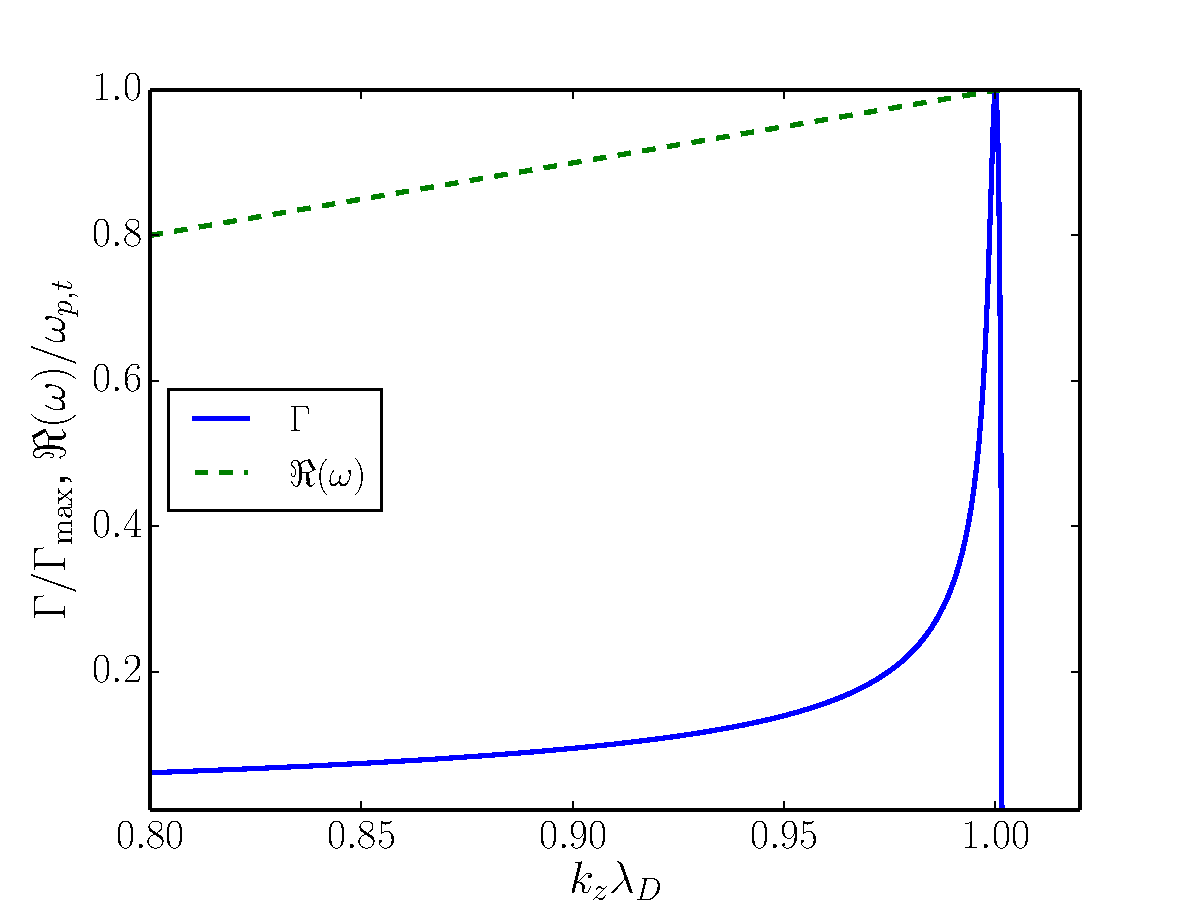
\includegraphics[width=0.5\textwidth]{off_res.pdf}
\caption{Beam-plasma growth rate (solid line) and unstable wave frequency (dashed-line) as a function of
  $k_z$ for $\gamma_b = 100$ and $n_b/n_t=10^{-3}$. \label{fig:OffResonance}}
\end{figure}


\subsection{Kinetic Instability}

The growth rate expressed in Equation (\ref{eq:growth rate reactive}) \cp{\sout{sits}is} in the reactive (or hydrodynamic) regime as the dispersion relation (Equation (\ref{eq:dispersion reactive})) could \cp{\sout{be}have} been derived from the fluid equations.  Here all the particles participate in the instability.  However, kinetic theory masks another regime of the instability, where only a fraction of the particle participate in the instability, i.e., the kinetic regime.  We now derive the growth rate of the instability in the kinetic regime.  

We begin first with the distribution function for the target plasma:
\begin{equation}
 F_t = \left(\frac{1}{2\pi m_e k_B T}\right)^{3/2}\exp\left(-\frac{p^2}{2m_e k_B T}\right),
\end{equation}
where the target plasma is assumed to be nonrelativistic, $\bmath{p}=m_e\vel$ is the nonrelativistic momentum,  and $T$ is the temperature of the background.
For the beam plasma, we adopt the Maxwell-J{\"u}ttner distribution (eq.~\ref{eq:distribution function beam}).
%\begin{equation}\label{eq:distribution function beam}
%F_b = \frac{n_b}{4\pi\gamma_b m^2 T K_2(m/T_{\rm L})} \exp\left(-\frac {\gammabeam(E - \betabeam \cdot \pmom)} {T}\right),
%\end{equation}
\cp{\sout{Plugging}Inserting} these into the dispersion relation (\ref{eq:dispersion relation}), we find
%\begin{equation}\label{eq:dispersion kinetic}
% 1 - \frac{\omega_{p,t}^2}{k}\int F_t\frac{k^2 - (\kvec\cdot\betavec)^2}{\gamma(\omega - \kvec\cdot\vel)^2} d^3p - \frac{\omega_{p,t}^2}{k}\int \frac{\kvec\cdot\gradp F_b}{\omega - \kvec\cdot\vel}d^3p  = 0,
%\end{equation}
\begin{equation}\label{eq:dispersion kinetic}
 1 - \frac{\omega_{p,t}^2}{k^2c^2}\int F_t\frac{k^2c^2 - (\kvec\cdot\vel)^2}{\gamma(\omega - \kvec\cdot\vel)^2} d^3p + \frac{m_e\omega_{p,b}^2}{k^2}\int \frac{\kvec\cdot\gradp F_b}{\omega - \kvec\cdot\vel}d^3p  = 0,
\end{equation}
where we have integrated by parts only the second term, associated with target plasma.  \cp{[Define $\gamma$, $\gamma_w$, $\gamma_b$, $\gamma_{\rm ph}$.]}

We discuss the solution to Equation (\ref{eq:dispersion kinetic}) in Appendix \ref{sec:solution kinetic}.  The associate growth rate for the kinetic beam plasma instability is  
\begin{equation}
\begin{aligned}
\Gamma &\simeq - \Gamma_0
\frac{\pi \gamma_w^2 \gph^3 m (\vph-v_{b,z'})}{4 \gamma_b \mu K_2(\mu) \cG'^3}\\
&\times\left[
\left( \cG'^2\mu^2 + 2\cG'\mu + 2 \right) 
+
\frac{\gamma_b^2 v_{b,x'}^2}{2\cG^2c^2} \left(2 \cG'\mu+ 2\right)
\right]
\exp(-\cG'\mu),\label{eq:kinetic growth rate}
\end{aligned}
\end{equation}
where $\Gamma_0 \equiv \omega_p \gamma_b (n_b/n_t) (m_e v_B^2/k_B T)$ is the typical maximum growth rate.  This specializes to the beam-plasma growth rate if we take $v_{b,x'} = 0$, which gives:
\begin{equation}
\Gamma_{\rm bp} \simeq - \Gamma_0
\frac{\pi \gamma_w^2 \gph^3 m (\vph-v_{b,z'})}{4 \gamma_b \mu K_2(\mu) \cG'^3}
\left( \cG'^2\mu^2 + 2\cG'\mu + 2 \right) 
\exp(-\cG'\mu),\label{eq:bp kinetic growth rate}
\end{equation}


\begin{figure}
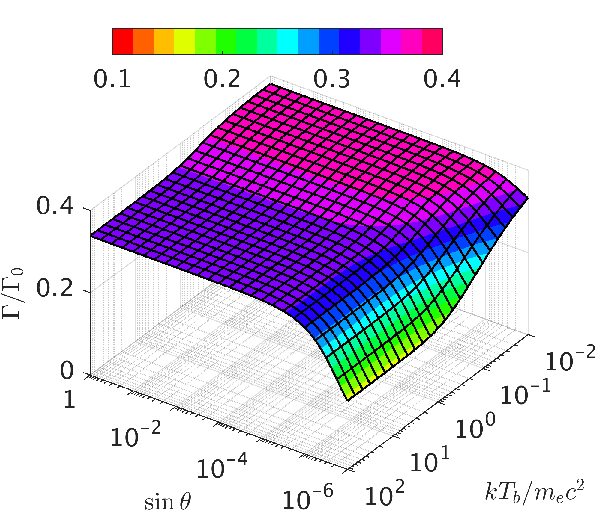
\includegraphics[width=0.5\textwidth]{pp1.pdf}
\caption{Oblique growth rate maximized over $\vph$ as a function of
  \cp{\sout{$v_{bx}$ and $T$}$\sin\theta$ and $k_BT/m_e c^2$, where $\theta$ is the angle between the beam direction and wave vector.\sout{ for various $\gamma_b$.
  In each the green line shows the chord along which $v_{bx}/v_b = 1/\gamma_b$.
  In all cases, the maximum growth rate occurs when
  $v_{bx}/v_b\gg1/\gamma_b$.}} \cp{[Which $\gamma_b$ was assumed for this -- $10^6$? Can you please add $k_B$ instead of $k$ to the axis label and $\Gamma/\Gamma_0$ at the color bar? In the paper, the notation $T$ is used instead of $T_b$ here -- can you unify this?]}}\label{fig:ObliqueGMZ}
\end{figure}

In Figure \ref{fig:ObliqueGMZ}, we plot the growth rate as a function of
\cp{$\sin\theta$, where $\cos\theta = \hat{\kvec}\cdot\hat{\vel}$} \sout{[is
    this correct?] $\cos\theta = \hat{k}\cdot\vel$}, i.e., the angle between the
beam and the wave vector, and $k_BT/m_e c^2$.  Here, it is clear that the growth
rate reaches it maximum value $\cos\theta \gg 1/\gamma_b$ \cp{[This is not
    clear, as the axis shows $\sin\theta$.]}, i.e., at an oblique, but not
perpendicular angle.  Moreover the maximum growth rates vary little and are
robust for broad range of angles between the wavevector and the beam direction.
Because the maximal oblique growth rate varies little for a wide range of angles
and relativistic temperatures for $k_B T/m_ec^2 > 1$, we maximize over $\theta$
in Figure \ref{fig:OGgen} and plot the maximal growth rate as a function of $T$
and $\gamma_b - 1$.  Here for relativistic beams, the maximum growth rate varies
little with $T$, varying by less than $10\%$ between hot and cold beams.  Thus,
we find:
\begin{equation}
\Gamma_M
\simeq
\left\{
\begin{aligned}
& 0.38 \Gamma_0 & k_BT/m_ec^2\ll 1\\
& 0.34 \Gamma_0 & k_BT/m_ec^2\gg 1
\end{aligned}
\right.\,,
\end{equation}
for $\gamma_b\gtrsim10$, as seen in Figure \ref{fig:OGgen}.  

\begin{figure*}
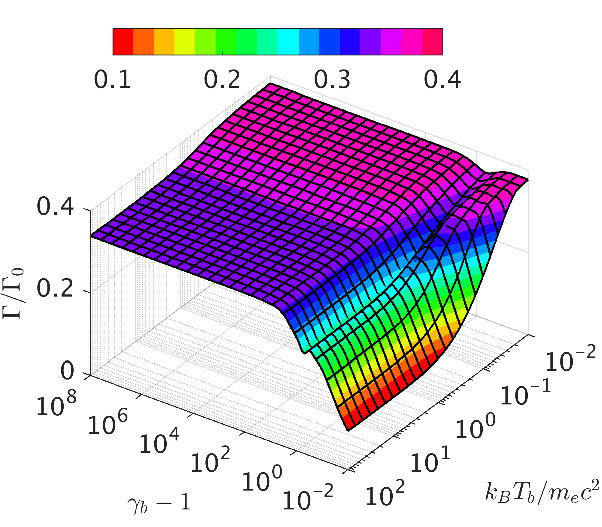
\includegraphics[width=0.5\textwidth]{pp2.pdf}
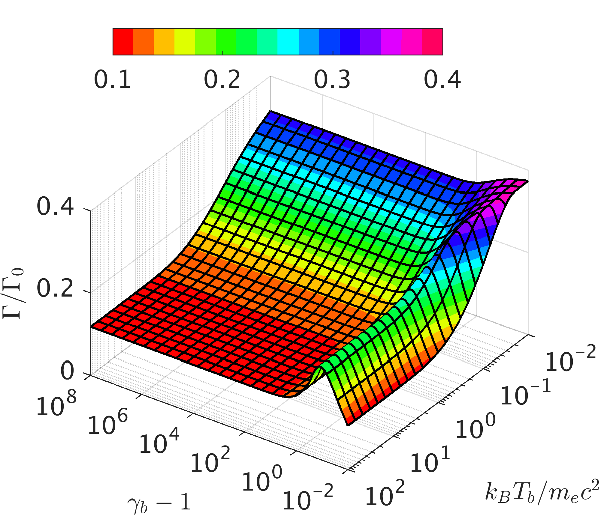
\includegraphics[width=0.5\textwidth]{pp3.pdf}

%\plottwo{pp2.pdf}{pp3.pdf}
\caption{Oblique kinetic growth rate (left) and beam-plasma growth rate (right),
  maximized over $\theta$ and normalized by
  $\Gamma_0\equiv\omega_{Pt}(n_b/n_t)\gamma_b m v_b^2/T$ as a function of
  $k_BT/m_ec^2$ and \cp{$\gamma_b-1$}.  \cp{\sout{Note that unlike the beam plasma case
      shown in Figure \ref{fig:Ggen}, at high $\gamma_b$ the transition between
      high and low temperature is only marginal, constituting a roughly $10\%$
      reduction.} Unlike the beam-plasma case on the right, in the case of the
    oblique kinetic growth rate at high $\gamma_b$ the transition between high
    and low temperature is only marginal, constituting a roughly $10\%$
    reduction.}  \cp{[Can you please add $k_B$ instead of $k$ to the axis label
      and $\Gamma/\Gamma_0$ at the color bar? In the paper, the notation $T$ is
      used instead of $T_b$ here -- can you unify this?]}} \label{fig:OGgen}
\end{figure*}

This can be contrasted with \cp{\sout{Figure~\ref{fig:bpgen}} the right panel of
  Figure~\ref{fig:OGgen}} where we plot the maximized beam-plasma growth rate
(\ref{eq:bp kinetic growth rate}) as a function of $\gamma_b - 1$ and $k_B
T/m_ec^2$.  Here, we see that the maximum growth rate is somewhat \cp{more}
sensitive to temperature, varying from $\Gamma/\Gamma_0 \approx 0.4$ for
$k_BT/m_ec^2 \ll 1$ to $\Gamma/\Gamma_0 \approx 0.1$ for $k_BT/m_ec^2 \gtrsim
1$.  Note, however, that that beam-plasma growth rate remains competitive with
the oblique growth rate, i.e., it is not orders of magnitude lower.
\cp{[Explain why we found the opposite result in Paper I, i.e., a negligible
    beam-plasma growth rate in comparison to the oblique growth rate.]}



% We discuss the solution to Equation (\ref{eq:dispersion kinetic}) in Appendix \ref{sec:solution kinetic}.  The associate growth rate for the kinetic beam plasma instability is  
% \begin{equation}\label{eq:growth-rate-bp}
%  \Gamma = -\frac{\sqrt{\pi} n_b\gamma}{n_t}\frac{\Delta\beta_{z,r}}{\sqrt{\alpha_{\parallel}}\alpha'_{\parallel}}\exp\left(-\frac{\Delta\beta_{z,r}^2}{\alpha_{\parallel}}\right),
% \end{equation}
% where $\alpha'_{\parallel} = \gamma^4\alpha_{\parallel}$ is the rescaled factor such that it is order unity.
% 
% In Figure \ref{fig:bp-growth-rate}, we plot the growth rate for the beam-plasma instability (eq.[\ref{eq:growth-rate-bp}]) for $\gamma^4\alpha_{\parallel} = 0.1, 0.3, 1,$ and 3.  The scaling of $\alpha_{\parallel}$ with $\gamma$ removes the overall scaling of $\alpha_{\parallel}$ with $\gamma$.  We have also parametrized the wavevector in terms of $\Delta k = k - k_0$, where $k_0 = \omega_{p,t}/v_b$ is the wavevector of the wave whose phase speed $v_{\rm ph} = v_b$ is equal to the speed of the beam.  Here in the limit of large $\gamma$, $\Delta v_{\rm ph}/v_{\rm ph} =  -\Delta k/k_0$, so the positive values of $\Delta k$ results in negative values of $\Delta v_{\rm ph}$, which puts these Langmuir waves in the rising part of the distribution function, i.e., $\partial F_2/\partial\Delta\beta_z > 0$, which is required for growth. Note as well that the maximum growth rate scales like $1/\gamma^4\alpha_{\parallel}$ in analogy with the scaling of $\Delta v^{-2}$ scaling in the non-relativistic case, where $\Delta v$ is the velocity dispersion \citep{Boyd}.   
% 
% The general solution for arbitrary $\kvec$ produces a growth rate of 
% \begin{eqnarray}
% \Gamma &=&  -\sqrt{\frac{\pi k_z}{k_x}}\frac{n_b\gamma}{n_t}\frac{\Delta\beta_{z,r}}{\sqrt{\alpha_{\perp}}}\frac{k_z}{k}\left(\frac{1}{\alpha'_{\perp}} + \frac{1}{\alpha'_{\parallel}} - \frac{k_z}{k_x\alpha'_{\parallel}}\right)\nonumber\\
% && \exp\left(-\frac{k_z^2\Delta\beta_{z,r}^2}{k_x^2\alpha_{\perp}}\right),\label{eq:growth-rate-oblique}
% \end{eqnarray}
% where $\alpha'_{\perp} = \gamma^2\alpha_{\perp}$ is an O(1) factor.  Again, we find that the overall scaling of the kinetic oblique instability is $\sim \gamma n_b/n_t$ like the kinetic beam plasma instability above.  Also we have made the assumption that $k_x/k_z \gg 1/\gamma$.  For $k_x/k_z < 1/\gamma$, the dispersion relation reverts back to the beam plasma case given in Equation (\ref{eq:growth-rate-bp})
% 
% % In Figure \ref{fig:oblique-growth-rate} we plot the growth rate for the oblique instability (eq.[\ref{eq:growth-rate-oblique}]) for $\alpha=\alpha'_{\perp} = \alpha'_{\parallel} = 0.1, 0.3, 1,$ and 3.  Here we have assumed that the perpendicular and parallel velocity dispersions are the same once the scaling for $\gamma$ has been removed.  This is true for small values of $\alpha$ that result from a rest-frame nonrelativistic distribution in Figure \ref{fig:distribution_non_rel}, but would not be the case for a rest frame relativistic distribution as shown in Figure \ref{fig:distribution_rel} where larger $v/c$ corrections come into play.  
% 
% Figure \ref{fig:oblique-growth-rate} also demonstrates that the oblique mode follows its name in that the fastest 
% growing mode is neither perfectly parallel ($k_x/k_z = 0$) nor perpendicular ($k_x/k_z = \infty$), but rather at a k-vector 
% where $k_x/k_z \sim O(1)$. This qualitatively matches the results of a full analysis of \citet{Bret-Grem-Beni:10}, who also found the greatest growth for nontrivial $k_x/k_z$. 
% 
% % \begin{figure}
% %  \includegraphics[width=0.5\textwidth]{bp-growth-rate.pdf}
% %  \caption{Growth rate for the relativistic kinetic beam-plasma instability (or bump on tail instability) for four different $\alpha'_{\parallel} = 0.1, 0.3, 1,$ and 3.  We choose to parametrized $\alpha_{\parallel}$ in this way to remove the scaling of $\alpha_{\rm parallel}$ with $\gamma$.  On the x-axis, we have plotted in terms of $\gamma^2\Delta k/k_0$, where $k_0 = \omega_{p,t}/v_b$ and $\Delta k = k - k_0$.  A Langmuir wave with $k=k_0$ moves at the exact speed of the beam.  For growth, Langmuir waves must move with a phase velocity $v_{\rm ph} < v_b$ to be on the rising part of the distribution function.  Hence, in the limit of large $\gamma$, $\Delta v_{\rm ph}/v_{\rm ph} =  -\Delta k/k_0$ where the extra factor of $\gamma^2$ is remove the scaling of $\Delta v_{\rm phase}$ with $\gamma$.  
% %  \label{fig:bp-growth-rate}}
% % \end{figure}
% 
% \begin{figure*}
%  \includegraphics[width=0.5\textwidth]{oblique-0_1.pdf}
%  \includegraphics[width=0.5\textwidth]{oblique-0_3.pdf}\\
%  \includegraphics[width=0.5\textwidth]{oblique-1.pdf}
%  \includegraphics[width=0.5\textwidth]{oblique-3.pdf}
%  \caption{Growth rate of the oblique instability for four different $\alpha=\alpha'_{\perp} = \alpha'_{\parallel} = 0.1, 0.3, 1,$ and 3. 1.  As in Figure \ref{fig:bp-growth-rate}, we choose to parametrized $\alpha_{\parallel}$ and $\alpha_{\perp}$ in this way to remove the scaling with $\gamma$.  On the x-axis, we have plotted in terms of $\gamma \Delta k/k_0$, for the same reasons as in Figure \ref{fig:bp-growth-rate}, but scaling with $\gamma$ instead of $\gamma^2$.  \label{fig:oblique-growth-rate}}
% \end{figure*}
% 

\subsection{The Transition between the Kinetic and Hydrodynamic Instability}\label{sec:transition}

The oblique instability exists in two different regimes, raising the important question: how are the two regimes related to each other. While this question has been studied by many authors in the context of the beam-plasma or two-stream instability \citep[see for instance][]{Melrose86,Boyd},  a clear exposition of how these two regimes are related to each other is lacking.  

To begin let us return to the reactive instability.  For the growth rate of the reactive instability (\ref{eq:growth rate reactive}) to be valid, the velocity dispersion $\rightarrow 0$.   To reach this limit, we demand
\begin{equation}
 \kvec\cdot\Delta \vel \ll \omega - \kvec\cdot\vel_b.
\end{equation}
Taking $\kvec$ to be $\omega_{p,t}/\vel_b$, so that the RHS is $\approx \Gamma$, we find
\begin{equation}\label{eq:oblique reactive regime}
 \frac{\Delta v_{\perp}}{v_b} \ll \left(\frac{n_b}{\gamma_b n_t}\right)^{1/3}
%\left(1 - \beta_b^2\cos^2\Psi\right)^{1/3}, 
\end{equation}
where we have dropped constant factors of order unity and assumed that $Z_x \sim O(1)$.  Hence, this defines the upper limit on the velocity dispersion of the plasma for the cold-plasma approximation to hold and, hence, the range of validity for the reactive oblique growth rate (\ref{eq:growth rate reactive}).  For $Z_x \ll \gamma^{-2}$, we recover the condition for the relativistic, reactive beam-plasma instability:
\begin{equation}\label{eq:bp reactive regime}
\frac{\Delta v_{\parallel}}{v_b} \ll \gamma_b^{-1}\left(\frac{n_b}{n_t}\right)^{1/3}.
\end{equation}

In Appendix \ref{sec:lorentz}, we estimate how the parallel and perpendicular velocity spreads scale in a Maxwell-Junter distribution.  The relevant results are: 
\begin{equation}
\frac{\Delta v_{\perp}^2}{c^2} \approx \frac {k_B T}{\gamma_b^2 m_e c^2 },
\end{equation}
and 
\begin{equation}
\frac{\Delta v_{\parallel}^2}{c^2} \approx \frac {k_B T}{\gamma_b^4 m_e c^2 },
\end{equation}
where $T$ is measured in the COM frame of the beam.  

Applying these results, we find
\begin{eqnarray}
\frac{\Delta v_{\perp}}{v_b} &\sim&  \gamma_b^{-1}\sqrt{\frac{k_BT}{m_ec^2}},\\
\frac{\Delta v_{\parallel}}{v_b} &\sim& \gamma_b^{-2}\sqrt{\frac{k_BT}{m_ec^2}}.
\end{eqnarray}
Hence, the conditions for the reactive regime for the oblique mode (eq.~\ref{eq:oblique reactive regime}) and beam-plasma mode (eq.~\ref{eq:bp reactive regime}) can be reduced to 
\begin{equation}\label{eq:generic reactive regime}
 \displaystyle
1 \ll \left\{
 \begin{array}{cl}
 ({k_BT}/{m_ec^2})^{-1/2}\gamma_b^{2/3}\left({n_b}/{n_t}\right)^{1/3} & \textrm{oblique} \\
({k_BT}/{m_ec^2})^{-1/2}\gamma_b\left({n_b}/{n_t}\right)^{1/3} & \textrm{beam plasma} 
\end{array}
\right..
\end{equation}

We now proceed to study the range of validity for the kinetic growth rate for the beam plasma mode (eq.~\ref{eq:bp kinetic growth rate}) and oblique mode (eq.~\ref{eq:kinetic growth rate}).  Following the argument of \cite{Boyd}, the growth occurs over a range where the distribution function is positive or $v_b - \Delta v < \omega/k < v_b$.  Hence the bandwidth over which the distribution powers grows is $\Delta \omega \sim k \Delta v$  For the beam plasma case, the growth rate is roughly
\begin{equation}
 \Gamma \sim \frac{n_b}{\gamma^3n_t} \left(\frac{c}{\Delta v_{\parallel}}\right)^{2}.
\end{equation}
The bandwidth, $\Delta \omega$, is then greater than the growth rate if 
\begin{equation}\label{eq:bp kinetic regime}
 \frac{\Delta v_{\parallel}}{v_b} \gtrsim \gamma^{-1}\left(\frac{n_b}{n_t}\right)^{1/3},
\end{equation}
which connects with the condition on the reactive beam plasma instability from Equation (\ref{eq:bp reactive regime}).
Similarly for the oblique mode, the bandwidth, $\Delta \omega$, is then greater than the growth rate if 
\begin{equation}\label{eq:oblique kinetic regime}
\frac{\Delta v_{\perp}}{v_b} \gtrsim \left(\frac{n_b}{\gamma n_t}\right)^{1/3},
\end{equation}
which can similarly compared to the condition on the reactive oblique mode from Equation (\ref{eq:oblique reactive regime}).

Combining these two kinetic condition and our result again from Section \ref{sec:setup}, we find  
\begin{equation}\label{eq:generic kinetic regime}
1 \ge \left\{
\begin{array}{cl}
({k_BT}/{m_ec^2})^{-1/2}\gamma_b^{2/3}\left({n_b}/{n_t}\right)^{1/3} & \textrm{oblique} \\
({k_BT}/{m_ec^2})^{-1/2}\gamma_b\left({n_b}/{n_t}\right)^{1/3} & \textrm{beam plasma} 
\end{array}
\right.,
\end{equation}
which in combination with Equation (\ref{eq:generic reactive regime}) denotes the transition between the reactive and kinetic regimes.

\section{Application to Ultrarelativistic $\epm$ Beams}\label{sec:application}

As discussed in the Introduction, the annihilation of VHEGRs and EBL photons produce ultrarelativistic \epm\ beams that are unstable to the beam plasma and oblique modes discussed above.  To apply the above results to the ultrarelativistic \epm\ beams, we now calculate their initial conditions.

\subsection{Average COM Energy of the \epm\ Beam}\label{sec:temperature}

To find the effective velocity dispersion of the ultrarelativistic \epm\ beam, we must first estimate the average COM energy of the beam.  To do so, we consider the process of photon-photon annihilation.  For a monoenergetic population of VHEGR photons with energy $E_{\rm ph}$, the production rate of \epm\ on EBL photons is
\begin{eqnarray}
\Gamma_{\pm}(E_{\rm ph}) &=& \int \sigma c dn_{\rm ebl} \nonumber \\
&=& \int \sigma\left(E_{\rm ph}, E_{\rm ebl}\right) c \frac{dn_{\rm ebl}}{dE_{\rm ebl}} dE_{\rm ebl},
\end{eqnarray}
where $\Gamma_{\pm}$ is the rate of pair production, $\sigma$ is the pair-production cross section, $n_{\rm ebl}$ is the number density of EBL photons, and $E_{\rm ebl}$ is the energy of the EBL photons.  There are two important components to this calculation -- the cross section, $\sigma$, and the spectra of the EBL.  

For $\sigma$, we use the results from \citet{Nikishov62} and \citet{Gould+67}, who considered a high energy photon with energy $E_{\rm ph}$ moving along the x-axis annihilating on an EBL photon with energy $E_{\rm ebl}$ moving at an angle, $\theta$, with respect to the x-axis.  The total cross section for this process is \citep{Nikishov62,Gould+67}
\begin{equation}\label{eq:cross section}
 \sigma = \frac {1}{2} \pi r_e^2\left(1-\frac{v_e^2}{c^2}\right)\left[\left(3-(v_e/c)^4\right)\ln\frac{1+v_e/c}{1-v_e/c} - 2\frac{v_e}{c}\left(2-\frac{v_e^2}{c^2}\right)\right],
\end{equation}
where $r_e = e^2/m_e c^2$ is the classical electron radius and $v_e$ is the electron velocity in the COM frame.  To find $v_e$, we use the energy of the electron in the COM frame, $E_e$, which is 
\begin{equation}
\label{eq:threshold}
 E_e =  \frac{m_e c^2}{1-v_e^2/c^2} = \sqrt{\frac{1}{2}{E_{\rm ebl} E_{\rm ph}\left(1-\cos\theta\right)}}.
\end{equation}
Pair production occurs when $E_e/m_e c^2 \geq 1$.

The second ingredient is the spectra of the EBL, which is not well constrained.  Here we use the constraints from \citet{Ahar_etal:06}, who demonstrated that VHEGR emission from H 2356-309 and 1ES 1101-232 places an upper limit on the EBL that is close to the lower limit of the integrated light from galaxies \citet{Madau+00}. Looking at Figure 1 of \citet{Ahar_etal:06}, we note that the EBL has a flat spectrum, i.e., constant ${dn_{\rm ebl}}/{dE_{\rm ebl}}$ below $1\,\eV$ and a falling spectrum  ${dn_{\rm ebl}}/{dE_{\rm ebl}}\propto E_{\rm ebl}^{-1.5}$ with a spectral index of $\approx 1.5$ above $1\,\eV$ with a rapid cutoff above $10\,\eV$. Thus, we adopt a simplified model:
\begin{equation}
 \frac{dn_{\rm ebl}}{dE_{\rm ebl}} \propto \left\{ 
\begin{array}{cl}
E_{\rm ebl}^0 & E_{\rm ebl} \leq 1\,\eV \\
E_{\rm ebl}^{-1.5} & 1\,\eV < E_{\rm ebl} \leq 10\,\eV \\
 0 & E_{\rm ebl} > 10\,\eV 
\end{array}
\right.
\end{equation}

In Figure \ref{fig:rates}, we plot the differential rate of pair production as a function of the COM energy of the electron (and positron) for a photon energy of $E_{\rm ph} = 0.3$ (dotted line), $1$ (solid line), $3$ (dash-dotted line) and $10\,\TeV$ (dashed line).  We use the COM energy in this case because in the COM frame, the energy of the EBL and TeV photon is the same and is $E_{\rm CM} = \sqrt{E_{\rm ebl}E_{\rm ph}}$ and $\theta \approx \pi - \sqrt{E_{\rm ebl}/E_{\rm ph}} \rightarrow \cos\theta = -1$\cp{ [What do you mean by $\theta\to\cos\theta$: this is not clear!]}, allowing us to ignore the dependence on $\theta$ in Equation (\ref{eq:cross section}).
We note several feature of this Figure.  First the distribution of COM energy for the electrons (and positrons) depends on the initial photon energy. This is because different energy photons probe different regimes of the EBL spectra.  Due to the rapid cutoff in the EBL above $10\,\eV$, lower energy VHEGRs produce colder beams.  This is seen in the average COM energies of the produced electrons, which are respectively, $E_e/m_e c^2 \approx 1.3, 1.6, 2$ and $3$ for $E_{\rm ph} = 0.3, 1, 3$ and $10\,\TeV$. Hence we expect that these pairs are in the sub-relativistic to mildly-relativistic regimes in their COM frame.
Second, the effect of the EBL spectra on the distribution of electron COM energies is also seen in the breaks in the distribution.  For instance, the cutoff in $d\Gamma_{\pm}/dE_{\rm ebl}$ above $E_e/m_e c^2 \approx 3$ for $E_{\rm ph} = 1\,\TeV$ is due to the cutoff in the EBL spectra above $10\,\eV$.  Additionally, the break in $d\Gamma_{\pm}/dE_{\rm ebl}$ at the same position for $E_{\rm ph} = 10\,\TeV$ is due to change in the EBL spectra at $1\,\eV$.  
\cp{[What $\Dpp$ does this correspond to?]}

\begin{figure}
 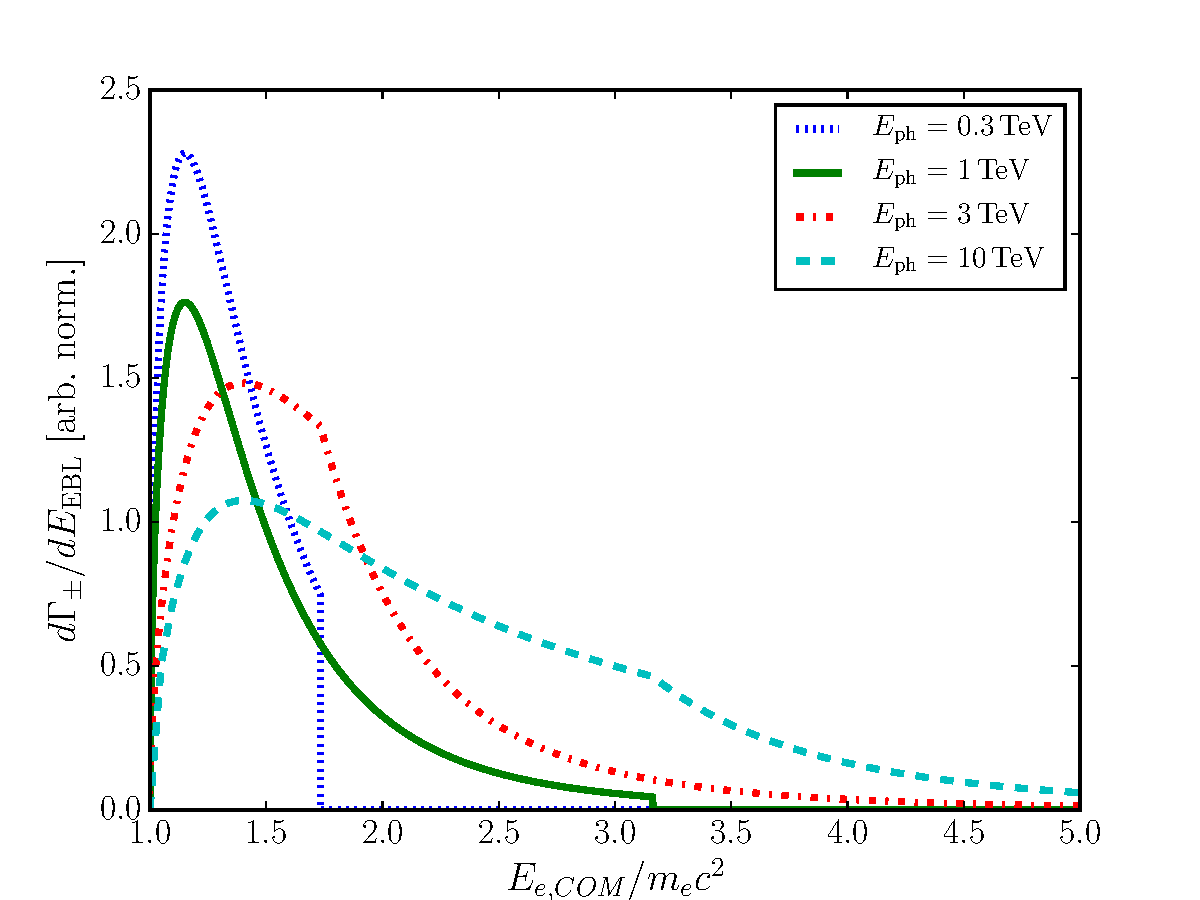
\includegraphics[width=0.5\textwidth]{rates.pdf}
 \caption{Differential rate of pair production as a function of the COM energy of the electron (and positron) for a photon energy of $E_{\rm ph} = 0.3$ (dotted line), $1$ (solid line), $3$ (dash-dotted line) and $10\,\TeV$ (dashed line).  The effect of the EBL spectra can be seen in different features in this plot.  The cutoff in $d\Gamma_{\pm}/dE_{\rm ebl}$ above $E_e/m_e c^2 \approx 3$ for $E_{\rm ph} = 1\,\TeV$ is due to the cutoff in the EBL spectra above $10\,\eV$.  The break in $d\Gamma_{\pm}/dE_{\rm ebl}$ at the same position for $E_{\rm ph} = 10\,\TeV$ is due to change in the EBL spectra at $1\,\eV$. The average COM energies of the produced electrons are $E_e/m_e c^2 \approx 1.3, 1.6, 2,$ and $3$ for $E_{\rm ph} = 0.3, 1, 3$, and $10\,\TeV$, respectively.  
 \label{fig:rates}}
\end{figure}

\subsection{Regime of Instability}

Given that the range of $E_e/m_e c^2$ between $1.3-3$ for $E_{\rm ph} = 1-10\,\TeV$, this corresponds to values of $\alpha_{\perp}'$ and $\alpha_{\parallel}'$ between $\sim 0.3-2$. \cp{[Define $\alpha_{\perp}'$ and $\alpha_{\parallel}'$.]}  To determine whether or not the reactive or kinetic instabilities apply to these beams, it is necessary to determine $n_b/n_t$.  Here the target is the background IGM, so $n_t = \nIGM$, where $\nIGM \approx 2\times 10^{-7}\,(1+\delta)\,(1+z)^3\,\cm^{-3}$ is the mean density of the IGM, $z$ is the redshift, and $\delta$ denotes the overdensity.  The number density of the TeV beam is more complicated as the production rate of pairs must be balanced against their loss due to plasma instabilities or ICC.  This is discussed extensively in Paper I and will not be repeated here.  However, we note that the important issue here is the loss rate due to plasma instabilities, which is a nonlinear process.  In Paper I, we assumed that the nonlinear loss rate was the same as the linear growth rate.  This remains to be shown and is the focus of ongoing work, of which this paper lays the initial foundation. 

Still some progress can be made if we assume that the dominant loss rate is ICC so that we can place a lower limit on the various plasma processes.  In this case, the ratio of the beam plasma density to the IGM, $n_b/\nIGM$, is then (Paper I):
\begin{eqnarray}
\frac{\nb}{\nIGM} &\simeq&
\frac{L_E}{2\pi\Dpp^3\GIC}\frac{1}{\nIGM} \\
&\simeq &
3\times10^{-18}
\left(\frac{1+z}{1}\right)^{3\zeta-7}
\left(\frac{E L_E}{10^{45}\erg\,\s^{-1}}\right)
\left(\frac{E}{\TeV}\right)
\,\cm^{-3}\,,\nonumber
\label{eq:nbIC}
\end{eqnarray}
where $L_E$ is the isotropic luminosity of the VHEGR source, $E$ is the energy of the VHEGR photon, $\Gamma_{\rm IC}$ is the inverse Compton cooling rate, and
\cp{\sout{$\Dpp$ is defined in the Introduction to be}} the mean free path of a VHEGR \cp{is given by
\begin{equation}
\Dpp(E,z) =
35 
\left(\frac{1+z}{2}\right)^{-\zeta}
\left(\frac{E}{1~{\rm TeV}}\right)^{-1}
~{\rm Mpc}\,,
\label{eq:Dpp}
\end{equation}
with $\zeta=4.5$ for $z<1$ and $\zeta=0$ for $z\ge1$ \citep{Knei_etal:04, Nero-Semi:09}.}

In Section \ref{sec:transition}, we derived the controlling parameter that delineates the reactive (eq.~\ref{eq:generic reactive regime}) and kinetic regimes (eq.~\ref{eq:generic kinetic regime}) by comparing the frequency spread of resonant waves, $\Delta\omega\sim k\Delta v$, with the growth rate, $\Gamma$.  Applying these conditions (eqns.~\ref{eq:generic reactive regime} and \ref{eq:generic kinetic regime}) to the ultrarelativistic $e^+e^-$ pair beams of interest, we find for the controlling parameter: 
\begin{eqnarray}
\frac{\gamma_b^{2/3}}{\sqrt{k_BT/m_e c^2}}\left(\frac{n_b}{\nIGM}\right)^{1/3} &=& 3.2\times 10^{-2} \frac{\gamma_6^{2/3}}{\sqrt{k_BT/m_e c^2}}\left(\frac{1+z}{2}\right)^{\zeta-7/3}\nonumber\\
&&\left(\frac{E L_E}{10^{45}\erg\,\s^{-1}}\right)^{1/3}
\left(\frac{E}{\TeV}\right)^{1/3},\label{eq:beam oblique condition}
\end{eqnarray}
and
\begin{eqnarray}
\frac{\gamma_b}{\sqrt{k_BT/m_e c^2}}\left(\frac{n_b}{\nIGM}\right)^{1/3} &=& 3.2 \frac{\gamma_6}{\sqrt{k_BT/m_e c^2}}\left(\frac{1+z}{2}\right)^{\zeta-7/3}\nonumber\\
&&\left(\frac{E L_E}{10^{45}\erg\,\s^{-1}}\right)^{1/3}
\left(\frac{E}{\TeV}\right)^{1/3}\label{eq:beam bp condition}
\end{eqnarray}
where $\gamma_6 = \gamma/10^6$. 
We see from our reactive (\ref{eq:generic reactive regime}) and kinetic (\ref{eq:generic kinetic regime}) conditions, that the oblique instability always exists in the kinetic regime, but the beam plasma instability \cp{\sout{sits}is} in the reactive regime at $z\gtrsim 1$ or for sufficiently cold beams $k_BT/m_e c^2 \lesssim 0.5$, which occurs \cp{for} $E_{\rm ph} \sim 1\,\TeV$ and for large $\gamma$, which occurs for $E_{\rm ph} \sim 10\,\TeV$ at $z=0$.  

The discussion above confirmed our earlier estimate in Paper I that the oblique instability \cp{\sout{sits}is} in the kinetic regime.  However, our new results suggest that the beam-plasma instability matches the oblique instability in effective growth rate in the kinetic regime and that the beam-plasma mode may also \cp{\sout{sit}exist} in the reactive regime.  However, we do not expect that the reactive beam-plasma mode will have a major effect on our earlier results.  First, plasma instabilities losses on the TeV pairs could easily push the beam plasma mode into the kinetic regime by reducing $n_b$, but this requires a proper estimate of the effect of the nonlinear instability.  This is a part of ongoing work and will be presented in a future publication. Second, while it seems that the beam plasma mode may \cp{\sout{sit}be} in the reactive regime, it is not too far from the kinetic regime, i.e., the controlling parameter, $({\gamma_b}/{\sqrt{k_BT/m_e c^2}})\left({n_b}/{\nIGM}\right)^{1/3}$, is order unity.  Thus, both the reactive and the kinetic growth rates are similar and \cp{it} likely makes little difference for the beam plasma mode which regime is assumed (in terms of growth rate).  Therefore, the use of the kinetic growth rate for the oblique mode (and beam-plasma mode)  in Paper I is valid, and the results of this paper buttresses the results of Paper I, II, III, and \citet{paperIV}.

\section{Summary and Conclusion}\label{sec:conclusions}

The ultrarelativistic $\epm$ beams that result from VHEGR-EBL annihilation are subject to powerful plasma beam instabilities including the beam plasma and oblique instability.  In this work, we \cp{\sout{have}examined} these linear instabilities as they would apply to the ultrarelativistic pair beams.  Our main findings are:
\begin{itemize}
%\item{We calculate how the parallel and perpendicular velocity dispersions of a distribution function responds under Lorentz boosts.  We show that these two velocities dispersions respectively scale like $\gamma^{-2}$ and $\gamma^{-1}$, allowing us to develop a simplified distribution function of the TeV electron-positron beam. We also show that this can be identified with a drifting relativistic Maxwell-J{\"u}ttner distribution. }
\item{We analytically calculated the beam-plasma and oblique instabilities in both the reactive and kinetic regime.  We have recovered the reactive scalings for the beam-plasma mode $\Gamma \sim \gamma^{-1}(n_b/n_t)^{1/3}$ and the oblique mode $\Gamma \sim (n_b/\gamma n_t)^{1/3}$.  In the kinetic regime, we have shown that the growth rate for both modes have the same scaling and similar normalization.}
\item{We also delineated the regime of applicability of the kinetic and reactive calculation and found, while the kinetic growth rates are similar for both the beam plasma and oblique mode, the condition for transition between the kinetic and reactive regimes \cp{\sout{for both}} are different.  In particular, the beam-plasma mode transitions at a lower value of $\gamma$ in comparison to the oblique mode.  This is due to a difference of $\gamma^{1/3}$ scaling between the two modes.}
\item{We calculate the average COM energy of the ultrarelativistic pair beam using a simplified model of the spectra of the EBL.  We found that the average energy of these beams range from $E_e/m_e c^2 = 1.3-3$ for $E_{\rm ph} = 1-10\,\TeV$, with colder beams at lower energies.  This is due to the rapid cutoff in the EBL above $10\,\eV$. }
\item{We demonstrate that the oblique mode is in the kinetic regime, while, the beam plasma mode is marginally in the reactive regime. In any case, the use of either regime produces roughly the same growth rate.  Moreover, the inclusion of plasma instability losses on the number density of beam particles may place the beam plasma mode firmly in the kinetic regime.}
\end{itemize}

%The results of this paper are a first step toward an understanding of the nonlinear regime of these plasma instabilities for ultrarelativistic \epm\ beams.  In particular, by developing a simple distribution function, whose modes can be analytically calculated, we will develop a quasilinear theory for these modes in a forthcoming publication.  Such a quasilinear calculation will capture the dominant wave-particle interaction and capture the initial nonlinear evolution of this instability.  

\acknowledgements
A.E.B.~and M.S.~receive financial support from the Perimeter
Institute for Theoretical Physics and the Natural Sciences and
Engineering Research Council of Canada through a Discovery Grant.
Research at Perimeter Institute is supported by the Government of
Canada through Industry Canada and by the Province of Ontario through
the Ministry of Research and Innovation.
PC is supported by the UWM Research Growth Initiative, the NASA ATP
program through NASA grant NNX13AH43G, and NSF grant AST-1255469.
C.P.~gratefully acknowledges support by the European Research Council under ERC-CoG grant CRAGSMAN-646955 and by the Klaus Tschira Foundation.
E.P. acknowledges support by the ERC grant ``The Emergence of Structure during the epoch of Reionization''.
We thank A. Bret for sharing his notes of the oblique instability and for extensive and enlightening discussions. 

%\onecolappendix
%\appendix%[onecolumn]
%\onecolumn
\begin{appendix}

\section{Lorentz Dependence of the Distribution Function and Velocity Dispersion}
\label{sec:lorentz}

Here we explicitly derive the scaling of the parallel and
perpendicular velocity dispersions with the Lorentz factor upon boosting the
distribution function to the lab frame. Let us begin with a distribution
function that is isotropic in the COM frame and depends only on energy.
Therefore in the COM frame, which we denote with the subscript ``CM'', the distribution
function is  $\fCM(E_{\rm CM}(\ppos_{\rm CM},\pmom_{\rm CM}))$.  When we move to the lab
(denoted with subscript ``L'') frame, the integral of the distribution function remains invariant,
i.e., total number, or
\begin{equation}
 \int \fLAB \dVLAB = \int \fCM \dVCM.
\end{equation}
It is well-known that under Lorentz transformations (Landau), 
\begin{equation}
 \dVLAB = \dVCM,
\end{equation}
so therefore,
\begin{equation}
  \fLAB(\ppos_{\rm L}(\ppos_{\rm CM},\pmom_{\rm CM}),\pmom_{\rm L}(\ppos_{\rm CM},\pmom_{\rm CM})) = \fCM(E_{\rm CM}).
\end{equation}

Now let us consider moments of the distribution function.  For clarity, it is helpful to consider moments of the distribution function first in the COM frame.  The velocity moment is (unsurprisingly):
\begin{equation}
 \betabarCM = \int \frac {\pmom_{\rm CM}}{\gamma_{\rm CM} mc} \fCM \dVCM = 0.
\end{equation}
We consider the lab frame to be  boosted along the x-axis by $\betaBOOST$. More precisely, the initial inertial frame is the COM frame and the lab frame is moving with velocity $\betaBOOST = -|\betaBOOST |$ with respect to the COM frame. This gives:
\begin{eqnarray}\label{eq:betabarLAB}
 \betabarLAB &=& \int \frac {\pmom_{\rm L}}{\gamma_{\rm L} mc} \fLAB \dVLAB  \nonumber\\
&=& \int \frac {\pmom_{\rm L}(\pmom_{\rm CM}, \ppos_{\rm CM})}{\gamma_{\rm L}(\pmom_{\rm CM}, \ppos_{\rm CM}) mc} \fCM \dVCM.
\end{eqnarray}
Breaking the components of \betabarLAB\ into components parallel and
perpendicular to the boost, we find: 
\begin{eqnarray}
\betabarLABpara &=& \int \frac{\betaCMpara -\betaBOOST}{1-\betaBOOST\betaCMpara} \fCM \dVCM,\\
\betabarLABperp &=& \int \frac{\betaCMperp}{\gamma_b\left(1-\betaBOOST\betaCMpara\right)} \fCM \dVCM,
\end{eqnarray}
where $\gamma_b = \left(1-\betaBOOST^2\right)^{-1/2}$ is the Lorentz factor of the boost between the lab and COM frame.  
For $\left|\betaCM\right|,\betaBOOST \ll 1$, we recover the Galilean invariant result, $\betabarLAB \approx \betabarCM - \betaBOOST\hat{\boldsymbol x}$.  
However, this Galilean result no longer holds for relativistic motion.

Now we consider the dispersion around $\betabar$.  In components, the COM frame is:
\begin{equation}
 \dbetabarCMi = \int \beta_i^2 \fCM \dVCM.
\end{equation}
In the lab frame, it is again useful to break it into components -- the parallel component becomes 
\begin{eqnarray}
  \dbetabarLABpara &=& \int (\beta_{\rm L, \parallel}-\betabarLABpara)^2 \fLAB \dVLAB ,\nonumber\\ 
 &=& \int \beta_{\rm L,\parallel}^2 \fLAB \dVLAB - \betabarLABpara^2,\nonumber\\
 &=&\int \left(\frac{\betaCMpara -\betaBOOST}{1-\betaMEAN^2}\right)^2 \fCM \dVCM - \betabarLABpara^2,\label{eq:dbetabarLABpara}
\end{eqnarray}
while the perpendicular component becomes
\begin{eqnarray}
 \dbetabarLABperp &=& \int \beta_{\rm L,\perp}^2 \fLAB \dVLAB, \nonumber\\
&=& \gamma_b^{-2} \int \frac{\betaCMperp^2}{\left(1-\betaMEAN^2\right)^2} \fCM \dVCM,
\label{eq:dbetabarLABperp}
\end{eqnarray}
where we have defined $\betaMEAN^2 = \betaCMpara\betaBOOST$ as the geometric mean for matters of convenience.  

It is easier to look at the perpendicular component first.  For $\left|\betaCM\right| \ll 1$, Equation (\ref{eq:dbetabarLABperp}) becomes to lowest order in $\betaCM$ 
\begin{equation}
 \dbetabarLABperp \approx \frac{\dbetabarCMperp}{\gamma_b^2} \approx \frac {k_B T}{\gamma_b^2 m_e c^2 }.
\end{equation}
This simple scaling of the perpendicular velocity dispersion can be understood as a scaling with time between two frames boosted relative to each other, where the coordinates perpendicular to the boost axis remain invariant.  This result is also in line with the transformation of temperature as $T\rightarrow T/\gamma$ under a boost, i.e., $mv^2 \sim kT$ -- two factors of $1/\gamma$ from the perpendicular velocity dispersion is countered by one factor of $\gamma$ from the mass.  Let us now consider the parallel component (eq.(\ref{eq:dbetabarLABpara})) again to lowest order in $\betaCM$: 
\begin{equation}
 \dbetabarLABpara \approx \frac{\dbetabarCMpara}{\gamma_b^{4}}  \approx \frac {k_B T}{\gamma_b^4 m_e c^2 },
\end{equation}
Here, the scaling of the parallel velocity dispersion can be understood as a double scaling of both time and coordinate (along the boost axis) between same two frames boosted relative to each other, giving an extra scaling of $\gamma^{-2}$.
This scaling of the parallel component of the velocity dispersion has important consequences that we explore in the main part of the paper.  



\section{Solution for the Reactive Regime}\label{sec:solution reactive}

This can be rewritten as 
\begin{eqnarray}\label{eq:dispersion reactive}
 \left(\omega^2 - \omega_{p,t}^2\right)\left[\left(\omega - k_z v_b\right)^2 - \frac{\omega_{p,b}^2}{\gamma^3}\frac{\gamma^2 k_x^2 + k_z^2}{k_x^2 + k_z^2}\right] = \frac{\omega_{p,t}^2\omega_{p,b}^2}{\gamma^3}\frac{\gamma^2 k_x^2 + k_z^2}{k_x^2 + k_z^2},
\end{eqnarray}
where we have added a factor of $\gamma^{-3}\omega_{p,t}^2\omega_{p,b}^2({\gamma^2 k_x^2 + k_z^2})/({k_x^2 + k_z^2})$ to both sides. 
To solve the dispersion relation (\ref{eq:dispersion reactive}), we take $\omega = \omega_{p,t} + \Delta\omega$ and expand to lowest order in
$\Delta\omega$ and $\omega_{p,b}$.  This gives
\begin{equation}
 2\Delta\omega\omega_{p,t}\left(\Delta\omega + \omega_{p,t} - k_z v_b\right)^2 = \frac{\omega_{p,t}^2\omega_{p,b}^2}{\gamma^3}\frac{\gamma^2 k_x^2 + k_z^2}{k_x^2 + k_z^2}.
\end{equation}\label{eq:expanded dispersion reactive}
For $\Delta\omega \ll \omega_{p,t} - k_z v_b$, $\Delta\omega$ is real and there is no instability.  However, if $k_z = \omega_{p,t}/v_b$, we then have
\begin{equation}\label{eq:approximate dispersion reactive}
 \Delta\omega^3 = \omega_{p,t}^3\frac{\omega_{p,b}^2}{2\gamma^3\omega_{p,t}^2}\frac{\gamma^2 Z_x^2 + 1}{Z_x^2 + 1},
\end{equation}
where we have multiplied the fraction on the right hand side by $(v_b/\omega_{p,t})^2/(v_b/\omega_{p,t})^2$ and $Z_x = k_xv_b/\omega_{p,t}$ is the dimensionless wavevector perpendicular to the beam direction.  
Equation (\ref{eq:approximate dispersion reactive}) gives three solutions for $\Delta\omega$: one real and two imaginary (one growing and one damping).  The maximum growth rate is then
\begin{equation}\label{eq:growth rate reactive appendix}
 \Gamma = \frac{\sqrt{3}}{2^{4/3}}\left(\frac{n_b}{n_t}\right)^{1/3}\left(\frac{\gamma^2 Z_x^2 + 1}{Z_x^2 + 1}\right)^{1/3}\frac{\omega_{p,t}}{\gamma}
\end{equation}

\section{Solution for the Kinetic Regime}\label{sec:solution kinetic}

As the target plasma is nonrelativistic, we can take $v\ll c$ and $\gamma \rightarrow 1$.  Expanding the denominator in powers of $v$, we find
\begin{eqnarray}
 \int F_t\frac{k^2c^2 - (\kvec\cdot\vel)^2}{\gamma(\omega - \kvec\cdot\vel)^2} d^3p &\approx& k^2c^2
 \int F_t \left(\frac {1}{\omega^2} + \frac {2\kvec\cdot\vel}{\omega^3} + \frac{3 (\kvec\cdot\vel)^2}{\omega^4}\right) d^3p \nonumber \\
&\approx& \frac {k^2c^2}{\omega^2}\left(1 + 3 {k^2\lambda_D^2}\right),
\label{eq:dispersion-real-part}
\end{eqnarray}
where the second term is zero because it is odd\cc{, $\lambda_D^2 = k_B T/m_e \omega_p^2$ is the Debye length, and we have assumed that $k^2\lambda_D^2 \ll 1$ and $\omega \approx \omega_p$ in the last term on the RHS\footnote{A direct solution to equation (\ref{eq:dispersion-real-part}) without approximating $\omega\approx \omega_p$ will reveal waves with nontrivial growth or damping rates.  These wave are not legitimate and result from the Taylor expansion of the denominator of equation (\ref{eq:dispersion-real-part}).  A correct treatment of equation (\ref{eq:dispersion-real-part}) with the appropriate Landau contours will give the correct growing or damping behavoirs for waves with phase speeds approximately that of the electron phase speeds.}}. If we ignore the third term in the kinetic dispersion relation (\ref{eq:dispersion kinetic}), this yields two plasma modes: an undamped plasma oscillation mode with $\omega = \omega_{p,t}$ and a longitudinal electron plasma wave, i.e., Langmuir wave, with
\begin{equation}
\omega \approx \omega_{p,t}\left(1 + \frac 3 2 k^2\lambda_{D,t}^2\right).
\end{equation}

To compute the contribution from the beam term, we will reorient our coordinate system and define the $z'$-axis along the wavevector, $\kvec$.  In this case we have the beam taking on a non-$z'$ component,  $\vel_b = v_{bz'}\zphat+v_{bx}\xphat$.   
This frame moves with a velocity, $\vel_{\rm ph} = \omega_k/k \zphat$.  With an eye toward computing the residue that will appear in equation (\ref{eq:dispersion kinetic}), we define $p_{z'}=\gz\vz E_\perp$, $E=\gz E_\perp$, and
$E_\perp=\sqrt{m^2+p_\perp^2}$ is the perpendicular energy.  In this case, we can rewrite the beam distribution function as
\begin{eqnarray}
F_B &=& \frac{m_e c^2}{4\pi\gamma_b k_B T K_2(m_ec^2/k_B T )m_e^3c^3} \exp\left(-\frac {\gamma_b(E - v_{b,z'} p_{z'} - v_{b,x'} p_{x'})} {k_B T}\right)\\
%F_b &=& \frac{1}{4\pi\gamma_b m^2 T K_2(m/T)} \exp\left(-\frac {\gammabeam(E - \betabeamz p_{z'} - \betabeamx p_{x'}}{T}\right),\label{eq:dist1}\\
&=& \frac{\mu m_e^{-3}c^{-3}}{4\pi\gamma_b K_2(\mu)}  \exp\left(-\frac {\gamma_b\gz(c^2 - v_{b,z'}v_{z'})E_\perp)} {k_BT c^2}\right)\exp\left(\frac{\gamma_bv_{b,x'} p_{x'}}{k_BT}\right),\label{eq:dist2}
\end{eqnarray}
where we define $\mu = m_ec^2/k_BT$.
\cp{\sout{Plugging}Inserting} the equation into (\ref{eq:dispersion kinetic}) and using the results of equation (\ref{eq:dispersion-real-part}), we find 
\begin{equation}
 1 - \frac{\omega_{p,t}^2}{\omega^2}\left(1 + 3 {k^2\lambda_D^2}\right) + i\frac{\pi n_b}{n_t}   m_e v_B^2 R = 0, 
\end{equation}
which involves the integral of 
\begin{equation}
R\equiv \int \frac{k\partial F_b/\partial p_{z'}}{\omega - k_{z'}v_{bz'}}d^3p,
\end{equation}
where $R$ is the residue for $p_{z'}$ such that $v_{z'} = v_{\rm ph}$.  

We can assume that $k\lambda_D \ll 1$ as the thermal velocity of the background plasma is much smaller than the speed of the ultrarelativistic beam.  We then take $\omega = \omega_r + i\Gamma$, where $\omega_r = \Re(\omega)$ is the real part of $\omega$ and the growth rate $\Gamma \ll \omega_r$, to find:
\begin{equation}
\Gamma \simeq -\omega_p\frac{\pi n_b}{2 n_t}   m_e v_B^2 R.
\end{equation}

Here two elements contribute to the pole:
\begin{equation}
\left.
\frac{\partial}{\partial p_{z'}} \left(\omega-k v_{bz'}\right)
\right|_{\rm pole}
=
\left.
- k \left(
  \frac{c^2}{E} - \frac{p_{z'}^2 c^4}{E^3}
\right)
\right|_{\rm pole}
=
- \frac{k c^2}{\gph^3 E_\perp}\,,
\end{equation}
and 
\begin{equation}
\begin{aligned}
\left.
k\frac{\partial F_b}{\partial p_{z'}}
\right|_{\rm pole}
%&=
&=
\left.
-\frac{k\gamma_b}{k_BT} \left( \frac{p_{z'} c^2}{E} - v_{b,z'}\right)
F_b
\right|_{\rm pole}\\
&=
-
\frac{
  k
  (\vph-v_{b,z'}) \mu^2}{
  4\pi m_e^{4}c^{5}K_2(\mu)
} \exp\left(-\frac {\gamma_b\gph(c^2 - v_{b,z'}v_{\rm ph})E_\perp)} {k_BT c^2}\right)\exp\left(\frac{\gamma_bv_{b,x'} p_{x'}}{k_BT}\right).
\end{aligned}
\end{equation}
%where we have used
%\begin{equation}
%\left.
%\gamma_b(E-v_{bz} p_z -v_{bx} p_x)/T
%\right|_{\rm pole}
%=
%\gamma_b \gph ( 1-v_{bz}\vph ) E_\perp/T - \gamma_b v_{bx} p_x/T\,.
%\label{eq:Eopole}
%\end{equation}

%and therefore,
%where $v_b\rightarrow v_{bz}$ and the only new term is the final
%exponential factor which depends upon $p_x$.

Putting this all together, the residue is
\begin{equation}
R
=
\frac{
  \gph^3 (\vph-v_{b,z'})\mu^2}{4\pi K_2(\mu)
}
\frac{\kI}{m_e^4c^7}
,
\label{eq:Rogen}
\end{equation}
where
\begin{equation}\label{eq:I-integral}
\kI \equiv \int d^2\!p_\perp E_\perp \exp\left(-\frac{\cG(E_\perp-w p_x)}{k_B T}\right)
\end{equation}
and $\cG\equiv\gamma_b\gph(1-v_{b,z'}\vph/c^2)$ and
$w\equiv \gamma_bv_{b,x'}/\cG \le 1$.  This latter inequality is guaranteed as 
\begin{equation}
\cG E_\perp - \gamma_b v_{b,x'} p_{x'} = \gamma_b(E - v_{b,z'} p_{z'} - v_{b,x'}p_{x'})|_{v_{b,z'}=v_{\rm ph}} > 0
\end{equation}
is the energy in beam frame and is therefore positive definite.  Noting that the $\exp(-wp_{x'})$ term appears as a boosted distribution, we boost by $w$
along the $x'$-axis, removing the anisotropic term from the
exponential.  

Thus, we define $p_{x'}'=\gamma_w(p_{x'}-w E_\perp/c^2)$ and $p_{y'}'=p_{y'}$ and find:
\begin{eqnarray}
%E'_\perp &=& \gamma_w(E_\perp - w p_x),\\
E_\perp &=& \gamma_w(E'_\perp + w p'_x),\\
d p_x d p_y &=& \frac{E_\perp}{E'_\perp} d p'_x d p'_y.
\end{eqnarray}
Inserting this into equation (\ref{eq:I-integral}), we find
\begin{equation}
\begin{aligned}
\kI &= 
\int d^2\!p'_\perp \frac{E_\perp^2}{E'_\perp} \exp\left(-\frac{\cG'E'_\perp}{k_B T}\right)\\
%&=
%\gamma_w^2 \int d^2\!p'_\perp \left(
 % E'_\perp + 2 w 
%\qc{p'_x}
%+ w^2 \frac{p'^2_x}{E'_\perp}
%\right) e^{-\cG'E'_\perp/m}\\
&=
\pi \gamma_w^2 \int_0^\infty dp'^2_\perp \left(
  E'_\perp + \frac{w^2}{2} \frac{p'^2_\perp}{E'_\perp}
\right) \exp\left(-\frac{\cG'E'_\perp}{k_B T}\right)\,,
\end{aligned}
\end{equation}
where $\cG'\equiv\cG/\gamma_w$. Note in the second line that we have used isotropy in $\bp_{\perp}'$ to eliminate terms linear in $\bp_{\perp}'$. 
% and in the second line we used the fact
%that  $E'_\perp e^{-\cG'E'_\perp/m}$ is isotropic in
%$\bp'_\perp$.  
Using the following integrals: 
\begin{equation}
\int_0^\infty dx \sqrt{1+x} e^{-a\sqrt{1+x}} = \frac{2 e^{-a}}{a^3}\left(a^2 + 2a + 2\right)
\end{equation}
and 
\begin{equation}
\int_0^\infty dx \frac{x}{\sqrt{1+x}} e^{-a\sqrt{1+x}}
=
\frac{4(a+1)}{a^3} e^{-a}\,,
\end{equation}
we find
\begin{equation}
\kI =
\frac{2 \pi \gamma_w^2 m_e^3c^4}{\cG'^3\mu^3} \left[
\left(\cG'^2\mu^2+2\cG'\mu+2\right)
+
\frac{w^2}{2c^2}
\left(2\cG'\mu+2\right)
\right]\exp\left(-\cG'\mu\right).
\end{equation}
Inserting this into (\ref{eq:Rogen}) yields
\begin{equation}
R = \frac{
  \gph^3 \gamma_w^2 (\vph-v_{b,z'}) 
}{ 2 \mu m_ec^2 \cG'^3 K_2(\mu)}
\left[
\left(\cG'^2\mu^2 + 2\cG'\mu + 2\right)
+
\frac{\gamma_b^2 v_{b,x'}^2}{2\cG^2 c^2} \left(2 \cG'\mu + 2\right)
\right] \exp\left(-\cG'\mu\right)
\end{equation}
and therefore,
\begin{equation}
\Gamma \simeq - \Gamma_0
\frac{\pi \gamma_w^2 \gph^3 m (\vph-v_{b,z'})}{4 \gamma_b \mu K_2(\mu) \cG'^3}
\left[
\left( \cG'^2\mu^2 + 2\cG'\mu + 2 \right) 
+
\frac{\gamma_b^2 v_{b,x'}^2}{2\cG^2c^2} \left(2 \cG'\mu+ 2\right)
\right]
\exp(-\cG'\mu),
\label{eq:OGgen}
\end{equation}
where $\Gamma_0 \equiv \omega_p \gamma_b (n_b/n_t) (m_e v_B^2/k_B T)$ is the typical maximum growth rate.
%The above differs from the beam plasma instability only due to the
%minor difference in the definition of $\cG'$ and the second term.  When
%$v_{bx}=0$, it is precisely the beam plasma instability growth rate.

%With an eye toward expanding to lowest order in $v_{bx}\ll1/\gamma_b\simeq1/\gph$, we find
%\begin{equation}
%\gamma_w 
%\simeq
%1 + \frac{v_{bx}^2}{2 \gph^2(1-v_{bz}\vph)^2}
%=
%1 + \frac{\gamma_b^2 v_{bx}^2}{2\cG^2}\frac{m^2}{T^2}
%\quad\Rightarrow\quad
%\cG'\simeq \cG - \frac{\gamma_b^2 v_{bx}^2}{2 \cG}\frac{m^2}{T^2}.
%\end{equation}  
%Thus, to lowest order in $\gamma_b v_{bx}$, equation (\ref{eq:OGgen}) becomes
%\begin{equation}
%\begin{aligned}
%\Gamma 
%&\simeq 
%- \Gamma_0
%\frac{\pi \gph^3 m (\vph-v_{bz})}{4 \gamma_b T K_2(m/T)}
%\frac{e^{-\cG}}{\cG^3}
%\left(
%  1
%  +
%  \frac{\gamma_b^2 v_{bx}^2}{\cG^2} \frac{m^2}{T^2}
%\right)\\
%&\qquad\times
%\left[
%\left( 
%  \cG^2 + 2\cG + 2 - \gamma_b^2 v_{bx}^2\frac{m^2}{T^2}  - \frac{\gamma_b^2 v_{bx}\qc{^2}}{\cG}\frac{m^2}{T^2}
%\right)
%+
%\frac{\gamma_b^2 v_{bx}^2}{2\cG^2} \frac{m^2}{T^2} \left(2 \cG + 2\right)
%\right]
%\\
%&\qquad\qquad\qquad\qquad\times 
%\left(
%  1 + 3 \frac{\gamma_b^2 v_{bx}^2}{2\cG^2}\frac{m^2}{T^2}
%\right)
%\left(
%  1 + \frac{\gamma_b^2 v_{bx}^2}{2\cG}\frac{m^2}{T^2}
%\right)\\
%&\simeq 
%- \Gamma_0
%\frac{\pi \gph^3 m (\vph-v_{bz})}{4 \gamma_b T K_2(m/T)}
%e^{-\cG}\\
%&\qquad\qquad\times 
%\left( 
%  \frac{\cG^2 + 2\cG + 2}{\cG^3}
%  +
%  \frac{\gamma_b^2 v_{bx}^2}{2}\frac{m^2}{T^2}
%  \frac{
%    \cG^3
%    +
%    5\cG^2
%    +
%    12\cG
%    +
%    12
%  }{\cG^5}
%\right)\,,
%\end{aligned}
%\end{equation}
%where $\Gamma_0\equiv \omega_{Pt} (n_b/n_t) \gamma_b m v_{bz}^2/T$, i.e.,
%again $v_{bz}$.

%However, obtaining asymptotic expansions for the growth rate in the high and
%low temperature limits that can be easily solved for the maximum
%growth rate is difficult.  Even with the tremendous numerical insight
%provided by Figure \ref{fig:ObliqueGMZ}, it is unclear how to make
%significant progress.  However, some general remarks can be made.  It
%appears at the maximum growth rate, we have to leading order:
%\begin{equation}
%\begin{gathered}
%\vph\simeq\sqrt{2\delta Z_x}\,,\quad
%v_{bx}=(1-\delta Z_x) v_b\,,\quad
%v_{bz}\simeq\sqrt{2\delta Z_x}\,v_b\,,\quad\\
%v_{bz}-\vph\simeq\left\{
%\begin{aligned}
%&\frac{\sqrt{T/m}}{\gamma_b} & T\ll m\\
%&\frac{1}{2\gamma_b} & T\gg m
%\end{aligned}
%\right.\,,\quad
%\gph\simeq1+\delta Z_x\,,\quad
%\cG' \sim \frac{m}{T}\,,\\
%\text{and}\quad w \sim 1\,,
%\end{gathered}
%\end{equation}
%\qc{[can you add more details which equations you approximate under which conditions? e.g., I get $1/2\gamma_b^2$ for the hot beam case \ldots]}\\
%where $\delta Z_x\equiv 1 - v_{bx}/v_b$.  Inserting these into Equation
%(\ref{eq:OGgen}) suffices to show that there exists growth rates that
%are $\propto \Gamma_0$, with 

%\begin{equation}
%\Gamma_M
%\simeq
%\left\{
%\begin{aligned}
%& 0.38 \Gamma_0 & T\ll m\\
%& 0.34 \Gamma_0 & T\gg m
%\end{aligned}
%\right.\,,
%\end{equation}
%for $\gamma_b\gtrsim10$, as seen in Figure (\ref{fig:ObliqueGMZ}).  
%

% We now proceed to the third term.  Without loss of generality, we orient our axes such that the beam is along the z-axis and the wavevector k sits in the x-z plane, i.e., $\kvec = k_x \xhat + k_z \zhat$. The beam distribution function (\ref{eq:distribution function beam}) now becomes
% \begin{equation}
% df=\frac{n_b}{\sqrt{\pi^3\dbetabarpara\dbetabarperp^2}}\exp\left(-\frac{\Delta \beta_{z}^2}{\dbetabarpara} - \frac{\Delta \beta_{x}^2 + \Delta\beta_{y}^2}{\dbetabarperp}\right) d^3\Delta\beta,
% \end{equation}
% We may integrate over $d\Delta\beta_y$ leaving an integral over $d\Delta\beta_z, d\Delta\beta_x$.  
% \begin{equation}\label{eq:integral1}
% \mathcal{I} = \int \frac{(k_x \partial_{p_x} + k_z\partial_{p_z}) F_1}{\omega - \kvec\cdot\vel}d\Delta\beta_z\, d\Delta\beta_x,
% \end{equation}
% where $F_1$ is the distribution function after has been integrated over $d\Delta\beta_y$.  Note that we have integrated the dispersion relation (\ref{eq:dispersion relation}) rather that the one that was integrated by parts (eq.[\ref{eq:dispersion relation by parts}]) because the Landau contour that we perform below is more explicit with this version.  Equation (\ref{eq:integral1}) can be rewritten as 
% \begin{equation}\label{eq:integral2}
% \mathcal{I} \approx \int \frac{(\gamma^2k_x\partial_{\Delta\beta_x} + k_z\partial_{\Delta\beta_z} ) F_1 d\Delta\beta_z\, d\Delta\beta_x}{k_z\gamma^3m_e c^2(\omega/k_z c - \beta_z - k_x\Delta\beta_x/k_z - \Delta\beta_z)}, 
% \end{equation}
% where we have converted the derivatives on $p_x$ and $p_z$ to derivatives on $\Delta \beta_x, \Delta \beta_z$ by assume that they are $ \ll 1/\gamma$ and $\ll 1/\gamma^2$, and take the following expansions:
% \begin{eqnarray}
%  p_x &\approx& 0 + \frac{\partial p_x}{\partial \Delta\beta_x} \Delta\beta_x \approx \gamma_{0} m_e c \Delta\beta_x\\
%  p_z &\approx& p_{z,0} + \frac{\partial p_z}{\partial \Delta\beta_z} \Delta\beta_z \approx p_{z,0} + \gamma_{0}^3 m_e c\Delta\beta_z,
% \end{eqnarray}
% where $\gamma_0 = \sqrt{1 + p_{z,0}^2/m_e^2c^2}$. 
%  
% \ac{[I had some difficulty with the above, in part because I think many approximations are being utilized at the same time.  Thus perhaps it would be better to explain each step in a bit more dtail.  
% The thing I had the most difficulty with was the $\bmath{p}\rightarrow\vel$ transformation in the integrands.  This is because the expansions in C6 \& C7 do not imply the transformation used in C5.  Rather, we should have
% \begin{equation*}
% \frac{\partial}{\partial p^j} 
% =
% \frac{\partial \beta^k}{\partial p^j} \frac{\partial}{\partial \beta^k}
% =
% \frac{\delta^k_j - \beta_j\beta^k}{\gamma m} \frac{\partial}{\partial \beta_k}\,,
% \end{equation*}
% and thus,
% \begin{equation*}
% \begin{aligned}
% \kvec\cdot\nabla_p F_1
% &=
% \frac{k^k - (k^j \beta_j)\beta^k}{\gamma m} \frac{\partial F_1}{\partial \beta_k}\\
% &=
% \frac{1}{\gamma m}
% \bigg\{
% \left[k_x - (k_x\beta_x+k_z\beta_z)\beta_x\right] \frac{\partial F_1}{\partial \beta_x}\\
% &\qquad\qquad
% +
% \left[k_z - (k_x\beta_x+k_z\beta_z)\beta_z\right] \frac{\partial F_1}{\partial \beta_z}
% \bigg\}\,.
% \end{aligned}
% \end{equation*}
% 
% When $k_x=0$, this simplifies a little bit, and we have
% \begin{equation*}
% \kvec\cdot\nabla_p F_1
% =
% \frac{1}{\gamma m}
% \left[
% -k_z\beta_z\beta_x\frac{\partial F_1}{\partial \beta_x}
% +
% k_z \left(1-\beta_z^2\right) \frac{\partial F_1}{\partial \beta_z}
% \right]\,,
% \end{equation*}
% and with $\beta_x\ll\beta_z\sim1$ we have
% \begin{equation*}
% \kvec\cdot\nabla_p F_1
% \simeq
% \frac{k_z}{\gamma^3 m}
% \left[
% -\gamma^2 \beta_z\beta_x\frac{\partial F_1}{\partial \beta_x}
% +
% \frac{\partial F_1}{\partial \beta_z}
% \right]\,,
% \end{equation*}
% with the important difference being the first term.  With the form of $F_1$ we have $\partial F_1/\partial \beta_j = 2\beta_j F_1 / \alpha_j$, and may evaluate each term to lowest order:
% \begin{equation*}
% \begin{aligned}
% &I_{x} \equiv -\int \frac{1}{\omega-k_z \beta_z} \frac{k_z}{\gamma^3 m} \gamma^2 \beta_z \beta_x 
% \left(\frac{2\beta_x}{\alpha_x} F_1\right)
% d\beta_x d\beta_z\\
% &\qquad\qquad= 
% -\int \frac{k_z \beta_z  F_2}{\gamma m (\omega-k_z \beta_z)} d\beta_z
% \simeq
% \left.-\frac{i \pi F_2}{\gamma m}\right|_{\beta_z=\omega/k_z}
% \\
% &I_{z} \equiv \int \frac{1}{\omega-k_z \beta_z} \frac{k_z}{\gamma^3 m} 
% \left[\frac{2(\beta_z-\beta_b)}{\alpha_z} F_1\right]
% d\beta_x d\beta_z\\
% &\qquad\qquad= 
% \int \frac{2 k_z (\beta_z-\beta_b) F_2}{\gamma^3\alpha_z m (\omega-k_z \beta_z)} d\beta_z
% \simeq
% \left.\frac{2 i \pi (\beta_z-\beta_b) F_2}{\gamma^3 \alpha_z m}\right|_{\beta_z=\omega/k_z}\\
% &\qquad\qquad\simeq
% - \frac{2(\omega/k_z-\beta_b)}{\gamma^2 \alpha_z} I_x\,.
% \end{aligned}
% \end{equation*} 
% Note that $I_{z}$ is just your expression C9.
% Now, since $\alpha_z\sim T/\gamma^4$, and $F_2$ is large for $|\omega/k_z-\beta_b|\lesssim\sqrt{\alpha_z}\sim T^{1/2}/\gamma^2$, $|I_z|\sim |I_x|/T^{1/2}$ and thus the neglected term is not generally small.
% 
% More problematic, I would like to understand why the $k_x=0$ case doesn't reproduce the standard cold plasma instability rate when $\alpha_z$ is very small.
% ]}
% 
% 
% 
% 
% 
% To make a connection with the the beam plasma instability, we take $k_x = 0$ and integrate Equation (\ref{eq:integral2}) over $d\Delta\beta_x$ to find:
% \begin{equation}\label{eq:integral-bp}
% \mathcal{I} \approx \frac{1}{\gamma^3 m_e c^2}\int \frac{\partial_{\Delta\beta_z} F_2}{(\omega/k c - \beta_z - \Delta\beta_z)}d\Delta\beta_z, 
%  \end{equation}
% where $F_2 = \sqrt{1/\pi\alpha_{\parallel}}\exp(-\alpha_{\parallel}^{-1} \Delta\beta_z^2)$ is the normalized distribution function after it has been integrated over $d\Delta\beta_x$.  Equation (\ref{eq:integral-bp}) can be evaluated using the Landau prescription, which yields a principle value (which is small and real and hence can be neglected as the background is dominant) and an imaginary component from the contribution of the pole
% \begin{equation}\label{eq:imaginary-bp}
%  \Im(\mathcal{I}) = \frac{i\pi}{\gamma^3 m_e c^2}\left.\frac{\partial F_2}{\partial\Delta\beta_z}\right|_{\Delta\beta_z = (\omega/k_z c - \beta_z)}
% \end{equation}
% 
% Combining equations (\ref{eq:dispersion kinetic}), (\ref{eq:dispersion-real-part}) and (\ref{eq:imaginary-bp}), we find
% \begin{equation}
%  \omega^2 - \omega_{p,t}^2\left(1 + 3k^2\lambda_D^2\right) - \frac{i\pi\omega_{p,b}^2\omega^2}{\gamma^3 k^2c^2}\left.\frac{\partial F_2}{\partial\Delta\beta_z}\right|_{\Delta\beta_z = (\omega/k_z c - \beta_z)} = 0.
% \end{equation}
% Expanding about $\omega = \omega_r - i\Gamma$ \cc{for $kc \approx \omega_r \approx \omega_{p,t}$ and assuming the imaginary parts is $O(\Gamma)$}, we find 
% \begin{eqnarray}\label{eq:growth-rate-bp-appendix}
%  \Gamma &=& \frac{\pi n_b}{2\gamma^3n_t}\left.\frac{\partial F_2}{\partial\Delta\beta_z}\right|_{\Delta\beta_z = (\omega/k_z c - \beta_z)}\omega_{p,t} \nonumber\\
%  &=& -\frac{\sqrt{\pi} n_b\gamma}{n_t}\frac{\Delta\beta_{z,r}}{\sqrt{\alpha_{\parallel}}\alpha'_{\parallel}}\exp\left(-\frac{\Delta\beta_{z,r}^2}{\alpha_{\parallel}}\right),
% \end{eqnarray}
% where $\alpha'_{\parallel} = \gamma^4\alpha_{\parallel}$ is the rescaled factor such that it is order unity.
% As $\Delta\beta_z \sim \sqrt{\alpha_{\parallel}}$, Equation (\ref{eq:growth-rate-bp}) has an overall scaling like $\gamma\nb/n_t$ in line scalings found for the kinetic oblique mode quoted in Paper I (also see below).  
% 
% We now assume $k_x \neq 0$ and perform the integral over $\Delta\beta_z$ in Equation (\ref{eq:integral2}) to find for the imaginary part
% \begin{equation}\label{eq:integral-kinetic}
%  \Im(\mathcal{I}) = \frac{i\pi}{\gamma^3 m_ec^2}\int \left(\gamma^2\frac{k_x}{k_z}\frac{\partial F_1}{\partial\Delta\beta_x} + \frac{\partial F_1}{\partial\Delta\beta_z}\right)_{\Delta\beta_z = \Delta\beta_{\rm res}} d\Delta\beta_x,
% \end{equation}
% where $\Delta\beta_{\rm res} = \omega/k_z c - \beta_z - k_x\Delta\beta_x/k_z$.  
% 
% To perform this integral, we write the exponent in $F_1$ as 
% \begin{eqnarray}
%  F_1 \sim \exp\left[\left(\frac 1 {\alpha_{\perp}} + \frac {(k_x/k_z)^2} {\alpha_{\parallel}}\right)\left(\Delta\beta_x - \left(1 - \frac{k_x^2\alpha_{\parallel}}{k_z^2\alpha_{\perp}}\right)\frac{\Delta\beta_{z,r}}{k_x/k_z}\right)^2 - \frac{\Delta\beta_{z,r}^2}{\alpha_{\parallel}} \right],
% \end{eqnarray}
% where the normalization $1/\pi\sqrt{\alpha_{\perp}\alpha_{\parallel}}$ has been left out and $\beta_{z,r} = \omega/k_zc - \beta_z$.  
% Making an appropriate substitution for $\Delta\beta_x \rightarrow \beta_x - \left(k_z/k_x - {k_x\alpha_{\parallel}}/{k_z\alpha_{\perp}}\right)\Delta\beta_{z,r}$, we find for Equation (\ref{eq:integral-kinetic}) 
% \begin{eqnarray}
% \Im(\mathcal{I}) = -\frac{i2}{\gamma^3 c}\sqrt{\frac{\pi k_z}{k_x\alpha_{\perp}}}k_z\left(\gamma^2\frac{1}{\alpha_{\perp}} + \frac{1}{\alpha_{\parallel}} - \frac{k_z}{k_x\alpha_{\parallel}}\right)\Delta\beta_{z,r}\exp\left(-\frac{k_z^2\Delta\beta_{z,r}^2}{k_x^2\alpha_{\perp}}\right) 
% \end{eqnarray}
% The resulting growth rate is then
% \begin{eqnarray}
% \Gamma = -\sqrt{\frac{\pi k_z}{k_x}}\frac{n_b\gamma}{n_t}\frac{\Delta\beta_{z,r}}{\sqrt{\alpha_{\perp}}}\frac{k_z}{k}\left(\frac{1}{\alpha'_{\perp}} + \frac{1}{\alpha'_{\parallel}} - \frac{k_z}{k_x\alpha'_{\parallel}}\right) \exp\left(-\frac{k_z^2\Delta\beta_{z,r}^2}{k_x^2\alpha_{\perp}}\right),\label{eq:growth-rate-oblique-appendix}
% \end{eqnarray}
% where $\alpha'_{\perp} = \gamma^2\alpha_{\perp}$ is an O(1) factor.  Again, we find that the overall scaling of the kinetic oblique instability is $\sim \gamma n_b/n_t$ like the kinetic beam plasma instability above.  Also we have made the assumption that $k_x/k_z \gg 1/\gamma$.  For $k_x/k_z < 1/\gamma$, the dispersion relation reverts back to the beam plasma case given in Equation (\ref{eq:growth-rate-bp})

\end{appendix}

\bibliography{bigmh}
\bibliographystyle{apj}


\end{document}


\ac{[The paragraph below is somewhat redundant now as the primary justifications have all been given above and in the appendix.  Plus there is the rather confusing redefinition of $\beta$ as well as the introduction of $v$.  I leave it here because I'm not quite sure what the point of it is, though believing that the main message is conveyed with my suggestion above.  Perhaps this could be an after-the-fact, more rigorous motivation for the above?  Is such a motivation necessary?  Could it be moved efficiently into the footnote (a potential minimal footnote is already now provided)?]
> > > > > > > > > > > > > > > > > >}
\begin{equation}
 f\propto\exp\left(-\frac{\left(v_{\parallel}-v_{\parallel,0}\right)^2}{\dbetabarpara}-\frac{v_{\perp}^2}{\dbetabarperp}\right),
\end{equation}
where $v_{\parallel} = p_{\parallel}/\gamma m_e c$ is the parallel velocity, $v_{\parallel,0} = p_{\parallel,0}/\gamma_0 m_e c \approx c$ is the velocity of the beam, and $v_{\perp} = p_{\perp}/\gamma m_e c$ is the perpendicular velocity.
To make further progress, we make the assumption that the spread in momentum $\ll p_{\parallel,0}$.  In other words, we assume that $\alpha_{\parallel}, \alpha_{\perp} \ll 1$.  In this limit, we can perform a Taylor expansion for $p_{\parallel}$ about $p_{\parallel,0}$ and $p_{\perp}$ about $0$.  
This gives: 
\begin{eqnarray}
 p_{\perp} &\approx& 0 + \frac{\partial p_{\perp}}{\partial v_{\perp}} \Delta v_{\perp} \approx \gamma_{0} m_e \Delta v_{\perp},\\
 p_{\parallel} &\approx& p_{\parallel,0} + \frac{\partial p_{\parallel}}{\partial v_{\parallel}} \Delta v_{\parallel} \approx p_{\parallel,0} + \gamma_{0}^3 m_e \Delta v_{\parallel},\\
 \gamma &\approx& \gamma_0 + \gamma_0^3 \frac{\Delta v_{\parallel}}{c}
\end{eqnarray}
where $\gamma_0 = \sqrt{1 + p_{\parallel,0}^2/m_e^2c^2}$. Hence this gives an approximate distribution function for a beam in terms of the perturbed velocities as 
\begin{equation}\label{eq:distribution function beam}
df=\frac{n_b}{\sqrt{\pi^3\dbetabarpara\dbetabarperp^2}}\exp\left(-\frac{\Delta \beta_{\parallel}^2}{\dbetabarpara} - \frac{\Delta \beta_{\perp}^2}{\dbetabarperp}\right) d\Delta\beta_{\parallel} d^2\Delta\beta_{\perp},
\end{equation}
where $\Delta\beta = \Delta v/c$ and we have assumed a 3-D geometry so that the perpendicular direction spans two dimensions: $\Delta\beta_{\perp}^2 = \Delta\beta_{\perp,1}^2 + \Delta\beta_{\perp,2}^2$.
This form of the distributions function (\ref{eq:distribution function beam}) has many of the properties of the Maxwell-Boltzmann distribution function, which we exploit below in our analytic calculations.
\ac{< < < < < < < < < < < < < < <}
